% !TEX program = xelatex
%% main.tex — 西南科技大学本科毕业论文
%% 题目：基于Spring Boot的AI Agent智能体编排系统的设计与实现
%% 编译命令：xelatex -shell-escape main.tex （运行两次生成正确交叉引用）

\documentclass[12pt, a4paper, openany]{ctexbook}
\usepackage{swust_thesis}
\usepackage{listings}
\usepackage{xcolor}
\usepackage{graphicx}
\graphicspath{{figures/}{./figures/}}
\usepackage{booktabs}
\usepackage{longtable}
\usepackage{float}
\usepackage{tikz}

%% 代码块全局样式
\lstset{
  basicstyle=\zihao{-5}\ttfamily,
  breaklines=true,
  frame=single,
  numbers=left,
  numberstyle=\tiny\color{gray},
  keywordstyle=\color{blue!80!black},
  commentstyle=\color{green!60!black},
  stringstyle=\color{red!70!black},
  tabsize=4,
}

\begin{document}

%% ========== 前置部分（罗马页码，无页眉）==========
\pagenumbering{Roman}
\fancypagestyle{frontmatter}{%
  \fancyhf{}%
  \fancyfoot[C]{\zihao{-5}\songti\thepage}%
  \renewcommand{\headrulewidth}{0pt}%
  \renewcommand{\headrule}{}%
}
\pagestyle{frontmatter}

%% 摘要（中英文）
%% 摘要

\cnabstract

随着大语言模型（LLM）推理能力的涌现，人工智能正经历从"被动响应工具"向"智能代理"的范式转变。
AI Agent 作为这一变革的核心载体，能够主动感知环境、规划路径、调用工具并执行复杂任务，
已成为大模型落地应用的关键技术方向。
然而，当前主流的 Agent 编排工具主要基于 Python 生态构建，难以与企业现有的 Java 微服务架构深度集成，
Java 开发者缺乏一套原生的、功能完备的 Agent 可视化编排平台。

针对上述问题，本文设计并实现了一套基于 Spring Boot 的 AI Agent 智能体编排系统。
系统采用领域驱动设计（DDD）的分层架构，融合 Spring AI 框架与可视化 DAG 编排能力，
围绕五项核心功能展开：Agent 管理与可视化编排、事件驱动的 DAG 工作流调度、
人工检查点与工作流恢复、知识库与检索增强、用户认证与系统安全支撑。

系统支持通过 React Flow 画布配置 Agent 工作流，并以 JSON 图结构持久化编排结果；
调度引擎基于"就绪节点驱动"策略执行 DAG，支持并行节点、条件分支和路径剪枝；
人工检查点机制允许审核人查看并修改中间结果后恢复流程，配合乐观锁和分布式锁保障并发安全。
同时，系统通过 MinIO 与 Milvus 完成文档存储、分块、向量化和语义检索，
并提供邮箱注册、登录、密码找回、验证码限流、BCrypt 加密和 JWT 令牌认证等安全能力。

系统前端基于 React + TypeScript 实现可视化流程编排与审核交互界面。
测试结果表明，系统五项核心功能链路已全面打通，核心接口响应延迟满足基本实时性要求，
具备 MVP 演示与业务验证能力。

\cnkeywords{AI Agent；智能体编排；Spring Boot；DAG 调度；人工检查点；领域驱动设计；知识检索增强}

\enabstract

With the rapid advancement of large language model (LLM) reasoning capabilities, artificial intelligence is undergoing a paradigm shift from \textit{passive response tools} to \textit{intelligent agents}. AI Agents, as the core carrier of this transformation, can proactively perceive environments, plan paths, invoke tools, and execute complex tasks, making them a key technical direction for deploying large models in practice. However, mainstream Agent orchestration tools are primarily built on the Python ecosystem, making deep integration with enterprise Java microservice architectures difficult. Java developers lack a native, fully-featured visual Agent orchestration platform.

To address this gap, this thesis designs and implements an AI Agent orchestration system based on Spring Boot. The system adopts a Domain-Driven Design (DDD) layered architecture and integrates Spring AI with visual DAG orchestration. It focuses on five core capabilities: Agent management and visual orchestration, event-driven DAG workflow scheduling, human checkpoint and workflow recovery, knowledge base retrieval augmentation, and user authentication with system security.

The system supports visual workflow configuration with React Flow and persists orchestration results as JSON graph definitions. The workflow engine adopts a ready-node-driven scheduling strategy and supports parallel execution, conditional branching, and path pruning. The human checkpoint mechanism allows reviewers to inspect and modify intermediate results before resuming execution, while optimistic locking and distributed locks ensure concurrent safety. In addition, MinIO and Milvus are used for document storage, chunking, vectorization, and semantic retrieval. The system also provides registration, login, password recovery, email verification, rate limiting, BCrypt encryption, and JWT-based authentication.

The frontend is implemented with React and TypeScript, providing an interactive visual workflow editor and review management interface. Testing demonstrates that all five core feature pipelines are fully operational with core API response latency meeting basic real-time requirements.

\enkeywords{AI Agent; Agent Orchestration; Spring Boot; DAG Scheduling; Human Checkpoint; Domain-Driven Design; Retrieval-Augmented Generation}

\clearpage


%% 目录
\clearpage
\tableofcontents

%% ========== 正文（阿拉伯页码，有页眉）==========
\clearpage
\pagestyle{fancy}
\pagenumbering{arabic}

%% 第1章 绪论

\chapter{绪论}

\section{选题背景及意义}

\subsection{选题目的}

随着大语言模型（Large Language Model，LLM）推理能力的涌现，人工智能正经历从"被动响应工具"
向"智能代理"（AI Agent）的范式转变。AI Agent 能够主动感知环境、规划路径、调用工具并执行
复杂任务，已成为大模型落地应用的关键技术方向。

为降低 Agent 的开发门槛，业界涌现出多种可视化编排平台。这些平台通过拖拽方式让开发者无需
编写大量胶水代码即可完成 Agent 工作流的设计，典型代表包括 Dify\upcite{dify2024}、Coze\upcite{coze2024}
等低代码平台，以及 LangGraph\upcite{langgraph2024}、AutoGen\upcite{wu2023autogen} 等开发框架。

然而，当前主流的 Agent 编排工具主要基于 Python 或 JavaScript 生态构建，难以与企业现有的
Java 微服务架构深度集成。在大规模、高并发、强类型的企业生产环境中，Java 生态的稳健性不可替代，
但 Java 开发者却缺乏一套原生的、功能完备的 Agent 可视化编排平台。

基于此背景，本研究旨在设计并实现一套\textbf{基于 Spring Boot 的 AI Agent 智能体编排系统}，
该系统融合 Spring AI 框架与可视化 DAG 编排能力，支持声明式配置、人机协作、知识增强与安全访问控制，
为 Java 开发者提供企业级的智能体开发解决方案。

\subsection{选题意义}

\textbf{在理论层面}，本研究探索声明式配置与 DAG 调度相结合的 Agent 编排方法。
当前 Agent 编排系统的研究多集中于 Python 生态，如何在 Java 环境下实现业务流程、知识检索、
人工审核与安全控制的一体化，仍缺乏系统性的工程化探索。本研究通过构建 Java 工程化系统，
为 AI Agent 在企业级场景中的落地提供新的实践参考。

\textbf{在应用层面}，本研究具有以下实用价值：
\begin{enumerate}
  \item 填补 Java 生态空白，使 Java 开发者能够利用现有技术栈进行 AI 应用开发；
  \item 通过可视化编排、DAG 调度和状态持久化机制，提高 AI 系统的可配置性与执行稳定性；
  \item 引入人工检查点、知识检索增强与认证安全机制，提升系统在企业场景下的可控性与可用性。
\end{enumerate}

\section{国内外研究现状}

\subsection{低代码 Agent 平台}

面向非技术用户的低代码平台发展迅速。国外以 Dify\upcite{dify2024}、Coze\upcite{coze2024}
等为代表，提供可视化的 Agent 搭建界面。国内方面，百度推出了 AgentBuilder，
阿里推出了 ModelScope-Agent，腾讯推出了元器等产品，均提供类似的低代码开发能力。

这类平台的优势在于入门门槛低，适合快速原型验证。但其局限性也很明显：
难以与企业现有的后端系统进行深度集成，只能通过 HTTP 端点等网络请求方式进行交互。

\subsection{Python 生态编排框架}

Python 生态处于领先地位。LangChain\upcite{langchain2023} 是目前最流行的 LLM 应用开发框架，
提供丰富的模型接口、工具集成和记忆管理能力，但早期"链式"设计在处理复杂循环逻辑时显得力不从心。

为解决这一问题，LangGraph\upcite{langgraph2024} 引入图论概念，将 Agent 的状态流转建模为节点与边的组合，
天然支持循环、分支和复杂流程控制，成为当前 Agent 工作流编排的重要方案。

微软研究院推出的 AutoGen\upcite{wu2023autogen} 则采用"对话即计算"范式，
让多个 Agent 以对话方式完成任务分解与协作，支持人机协作和代码执行等功能。

上述 Python 框架功能强大，但对 Java 开发者存在较高的学习和集成门槛，
难以直接应用于企业现有的 Spring Boot 微服务架构中。

\subsection{Java 生态现状}

Spring AI\upcite{springai2024} 作为 Spring 官方推出的 AI 应用框架，在近期逐步成熟，
提供了统一的模型接口（ChatClient）、结构化输出和函数调用机制，但目前主要解决 LLM 接入层面的问题，
尚未提供成熟的工作流编排能力。

Java 生态中缺乏一个类似 LangGraph 的、基于配置驱动的图导向编排引擎，
开发者仍需手动编写大量代码来管理 Agent 的状态流转和任务调度。\textbf{这一空白正是本研究的切入点。}

\section{研究目标与内容}

\subsection{研究目标}

本研究的目标是设计并实现一套基于 Spring AI 的 AI Agent 编排系统，
围绕企业级智能体应用的配置、执行、审核、增强与安全支撑需求，形成以下五项核心能力：

\textbf{（1）Agent 管理与可视化编排：}系统支持通过可视化画布拖拽节点、配置参数与连接关系，
以 JSON 图结构保存 Agent 工作流，并支持版本发布、回滚与管理。

\textbf{（2）工作流调度执行：}系统支持基于 DAG 的事件驱动调度，
实现节点并行执行、条件分支、路径剪枝与状态推进。

\textbf{（3）人工审核与恢复机制：}系统支持在关键节点引入人工检查点，
实现暂停、查看上下文、修改中间结果、审批恢复或拒绝终止。

\textbf{（4）知识库与检索增强：}系统支持文档上传、切分、向量化入库与语义检索，
在工作流执行过程中为 LLM 节点注入外部知识上下文。

\textbf{（5）用户认证与系统安全支撑：}系统支持邮箱注册、登录、找回密码和令牌认证，
并通过验证码频率控制、密码加密与访问控制保障系统安全。

\subsection{研究内容}

研究内容分为四个板块：

\textbf{（1）需求分析：}分析 Java 开发者、业务人员、系统管理员等角色的使用场景，
围绕 Agent 管理、工作流执行、人工审核、知识检索与用户认证构建需求模型。

\textbf{（2）系统设计：}采用 DDD 分层架构思想，设计前后端分离与领域驱动相结合的系统结构，
明确可视化编排、执行调度、审核恢复、知识处理与认证安全等模块之间的数据流与职责边界。

\textbf{（3）功能实现：}重点实现 Agent 管理与可视化编排、工作流调度执行、人工检查点与恢复、
知识库与检索增强、用户认证与系统安全支撑五个核心模块。

\textbf{（4）系统测试：}覆盖单元测试、集成测试和功能测试三个层面，
验证五个核心模块的功能闭环与关键链路可用性。

\section{本章小结}

本章阐述了本文的选题背景与研究意义，综述了低代码 Agent 平台、
Python 编排框架和 Java 生态的国内外研究现状，
明确了本文面向 Java 生态的研究定位，并将研究目标统一收束为
Agent 管理与可视化编排、工作流调度执行、人工审核与恢复机制、
知识库与检索增强、用户认证与系统安全支撑五个核心模块，
为后续研究工作奠定了背景基础。
           %% 第1章 绪论
%% 第2章 AI Agent 智能体编排系统需求分析

\chapter{AI Agent 智能体编排系统需求分析}

\section{系统功能需求分析}

\subsection{功能需求描述}

系统面向三类用户角色：Java 开发者（API 集成与配置）、业务人员（可视化编排与审批）
和系统管理员（运维与监控）。系统用例图如图~\ref{fig:use_case}~所示。

\begin{figure}[H]
  \centering
  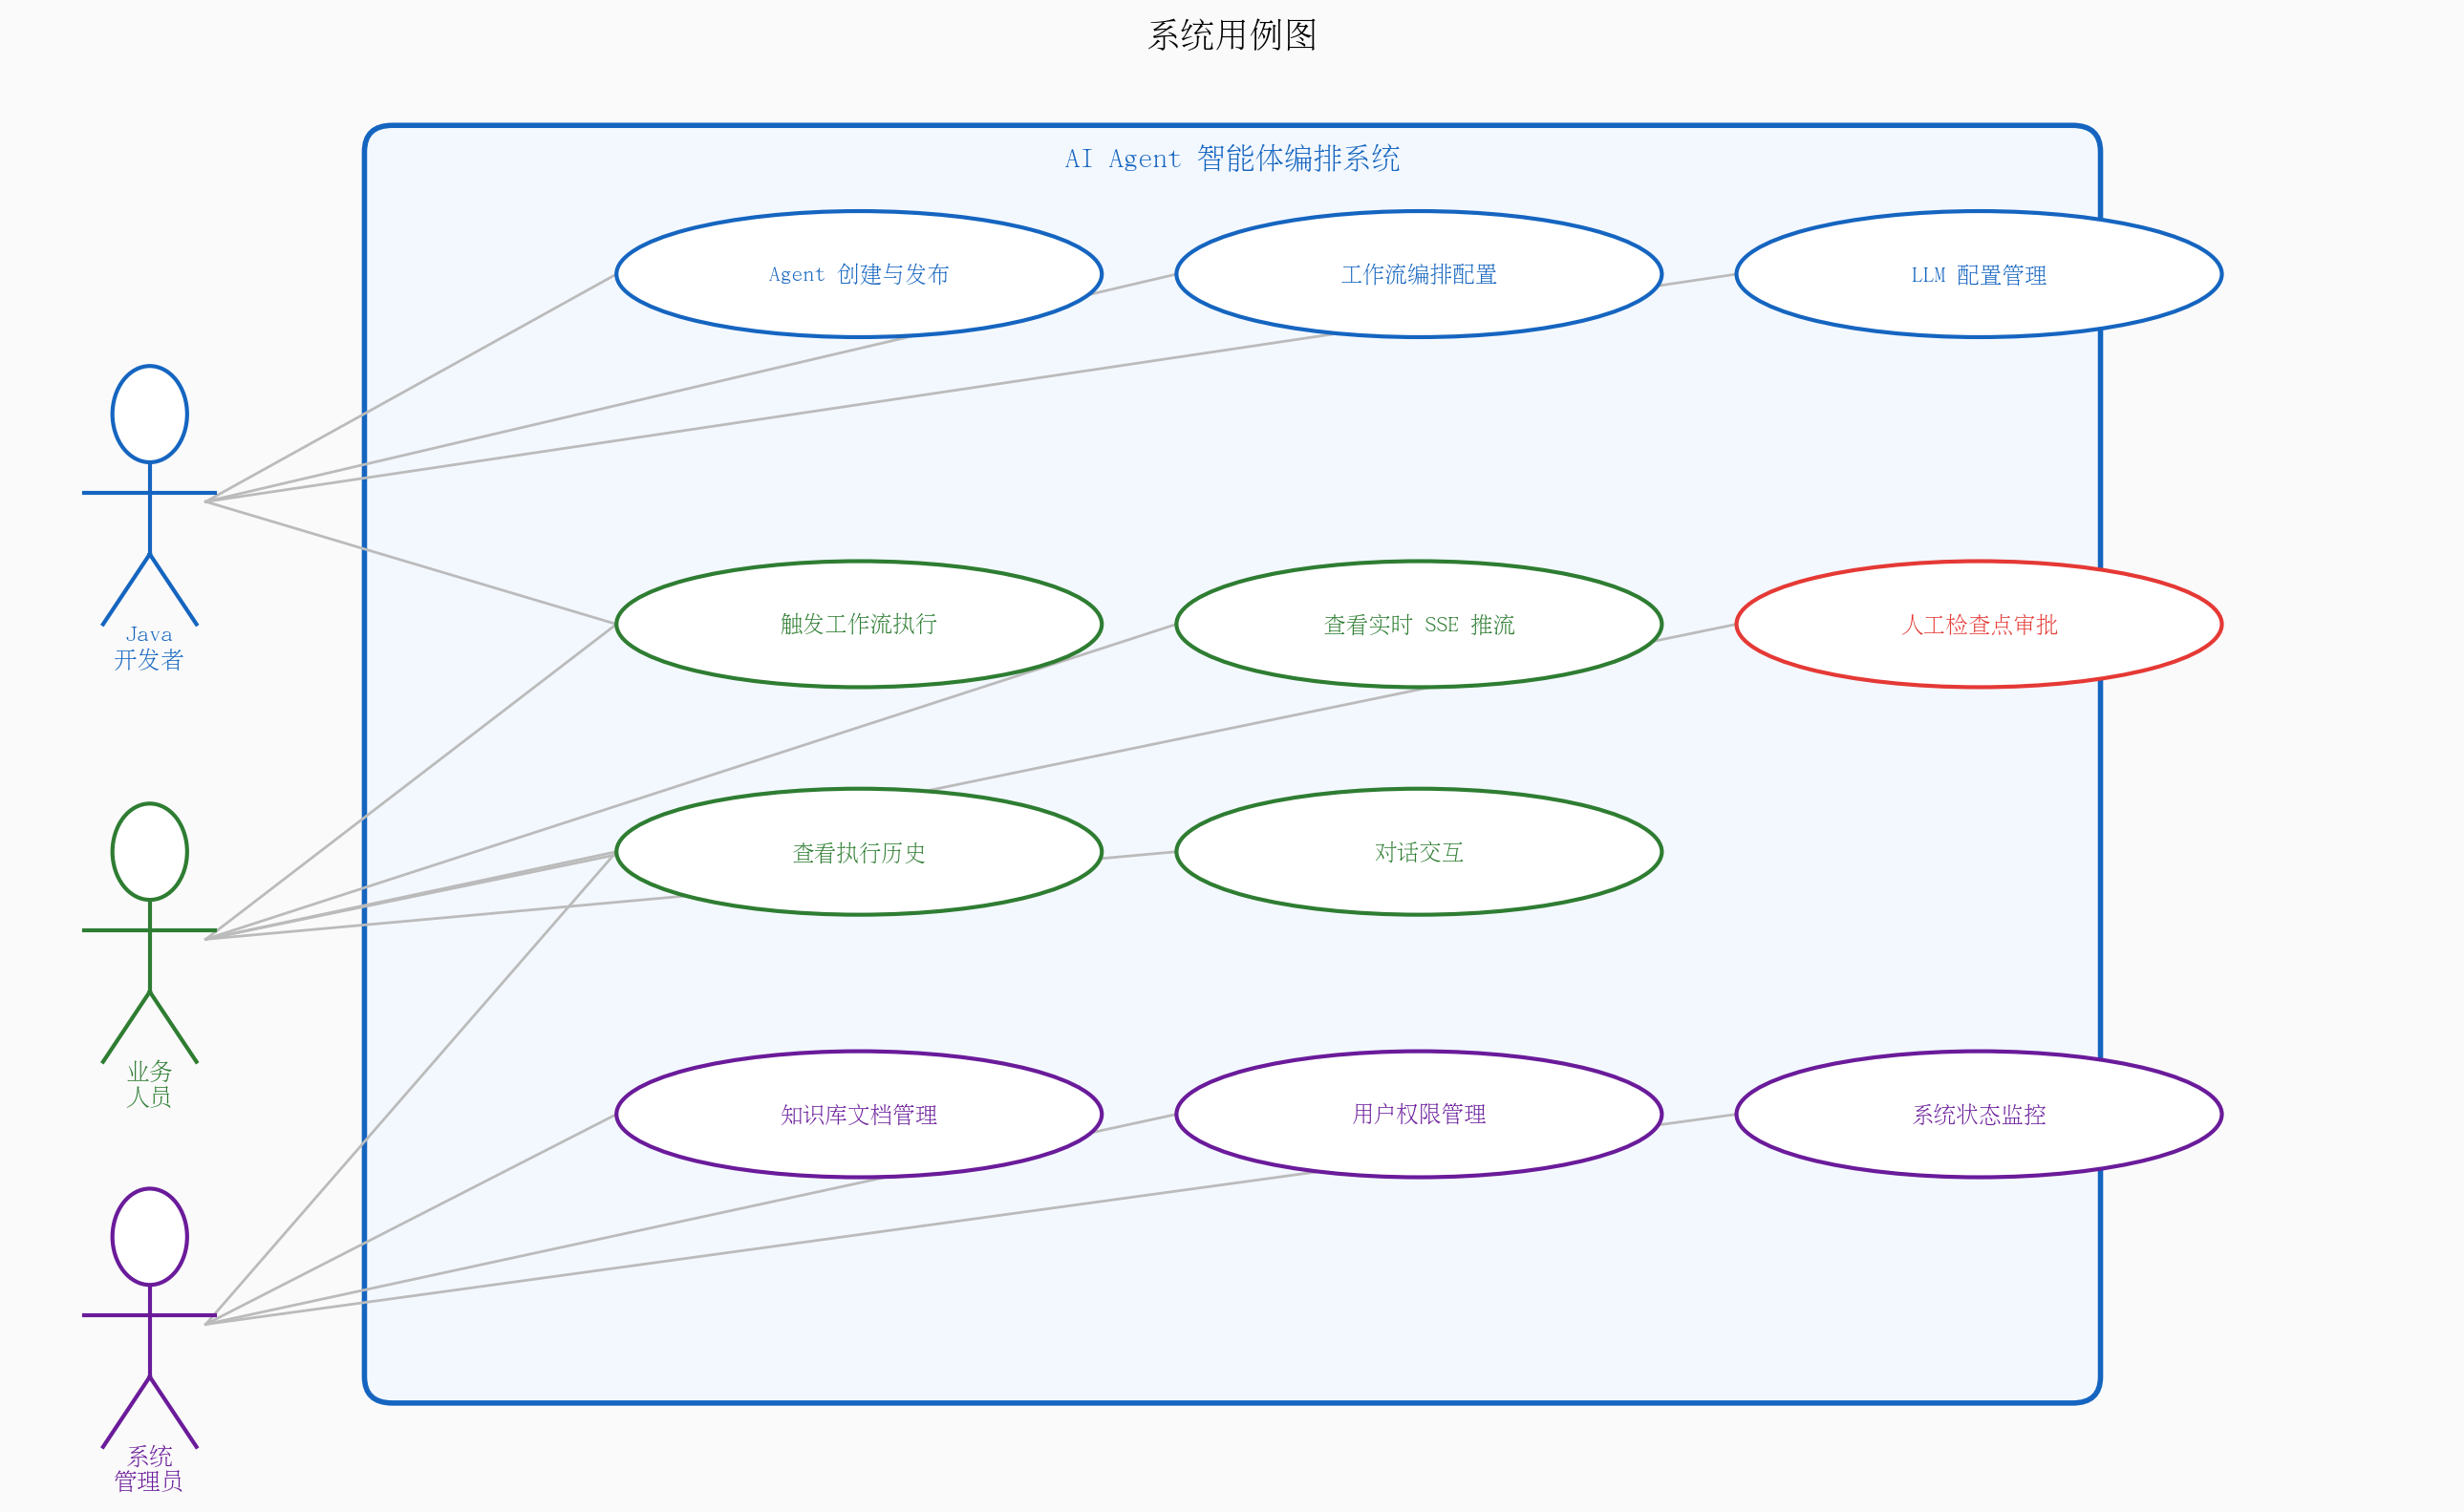
\includegraphics[width=0.95\textwidth]{figures/fig_usecase.png}
  \caption{系统用例图}
  \label{fig:use_case}
\end{figure}

围绕论文最终确定的五个核心模块，系统功能需求可归纳如下：

\subsubsection{（1）Agent 管理与可视化编排需求}

系统需要支持 Agent 的全生命周期管理，包括创建、编辑、发布、版本查询与回滚。
用户可维护 Agent 的基础信息（名称、描述、图标）以及底层工作流图定义。
在前端，业务人员通过可视化画布拖拽节点、配置参数、建立边连接，
并将画布状态保存为 JSON 图结构。系统需保证草稿态与发布态隔离，
避免开发中的修改直接影响线上运行中的 Agent。

\subsubsection{（2）工作流调度执行需求}

系统需要支持基于 DAG 的工作流执行能力。用户在对话界面输入任务后，
系统应根据 Agent 配置解析工作流图，完成节点状态初始化、拓扑调度、条件分支处理、
并行节点执行和最终结果汇总。执行过程中需要实时输出节点运行进度和模型生成结果，
并保证执行状态可查询、执行日志可追溯。

\subsubsection{（3）人工审核与恢复机制需求}

系统需要在关键节点引入人工检查点机制。当工作流执行到指定节点时，
可根据 BEFORE\_EXECUTION 或 AFTER\_EXECUTION 两种阶段自动暂停，
等待审批人查看输入或输出内容后进行决策。审批人可通过审批页面选择通过或拒绝，
并在通过前对中间结果进行修正。系统需记录审批人、审批时间、修改内容和拒绝原因，
满足合规审计要求，同时在多人并发审批时保障状态一致性。

\subsubsection{（4）知识库与检索增强需求}

系统需要支持知识数据集管理、文档上传、分块处理、向量化入库和检索增强。
用户可上传 PDF、Word、TXT、Markdown 等多种格式文档，系统对文档进行解析与分块后，
调用嵌入模型将文本块写入 Milvus 向量数据库。运行时，工作流中的知识节点或检索接口
应能够根据用户问题进行语义搜索，返回 Top-K 相关内容作为上下文，增强大模型回答质量。

\subsubsection{（5）用户认证与系统安全支撑需求}

系统需要提供用户注册、登录、找回密码和身份认证能力。
注册与重置密码需依赖邮箱验证码校验；登录后系统应签发访问令牌，
保证 Agent 管理、知识库管理、工作流执行与审批操作均运行在已认证用户上下文中。
同时，系统应具备验证码发送频率限制、登录失败限流、密码加密存储和访问审计等安全能力。

\subsection{主要用例详细描述}

在系统所有功能中，Agent 管理与编排、工作流执行、人工审核、知识检索和用户认证构成了核心闭环。
以下选取其中五个代表性用例进行详细说明。

\subsubsection{（1）Agent 创建与发布}

表~\ref{tab:uc_agent}~为 Agent 创建与发布用例的需求说明表。

\begin{table}[H]
  \centering
  \caption{Agent 创建与发布用例需求表}
  \label{tab:uc_agent}
  \begin{tabular}{|p{3cm}|p{10cm}|}
    \hline
    \textbf{用例标识} & UC-01 Agent 创建与发布 \\
    \hline
    \textbf{功能描述} & 用户创建 Agent、在可视化画布中完成编排并发布可执行版本 \\
    \hline
    \textbf{使用人员} & Java 开发者 / 业务人员 \\
    \hline
    \textbf{前置条件} & 用户已登录，具有 Agent 管理权限 \\
    \hline
    \textbf{输入} & Agent 基础信息、节点配置、边连接关系、图结构 JSON \\
    \hline
    \textbf{系统响应} & 创建初始 Agent，保存 graphJson，校验图结构并生成版本快照 \\
    \hline
    \textbf{输出} & 返回 Agent ID、最新版本信息和发布结果 \\
    \hline
    \textbf{操作序列} & 用户创建 Agent 并进入画布编排，保存草稿后发布版本，系统写入版本快照 \\
    \hline
    \textbf{异常} & 图结构存在环路 → 拒绝保存；版本冲突 → 提示重新加载草稿 \\
    \hline
  \end{tabular}
\end{table}

\subsubsection{（2）工作流执行}

表~\ref{tab:uc_exec}~为工作流执行用例的需求说明表。

\begin{table}[H]
  \centering
  \caption{工作流执行用例需求表}
  \label{tab:uc_exec}
  \begin{tabular}{|p{3cm}|p{10cm}|}
    \hline
    \textbf{用例标识} & UC-02 工作流执行 \\
    \hline
    \textbf{功能描述} & 用户输入任务，触发 Agent 工作流执行，实时接收 SSE 推送的进度和结果 \\
    \hline
    \textbf{使用人员} & Java 开发者 / 业务人员 \\
    \hline
    \textbf{前置条件} & Agent 已发布，工作流配置完整，DAG 无环 \\
    \hline
    \textbf{输入} & 用户消息（input/query/message）、agentId、conversationId（可选） \\
    \hline
    \textbf{系统响应} & 解析 Agent 图定义，加载检索增强上下文与会话历史，初始化执行上下文，DAG 拓扑调度 \\
    \hline
    \textbf{输出} & 通过 SSE 推送节点启动/完成/错误事件和 LLM 流式输出 delta；执行完成后返回最终结果 \\
    \hline
    \textbf{操作序列} & 用户发送消息后建立 SSE 连接，调度器按图结构执行节点并持续推送执行事件 \\
    \hline
    \textbf{异常} & 节点执行失败 → 推送 error 事件，整体状态变为 FAILED；DAG 含环 → start() 抛异常，返回 400 \\
    \hline
  \end{tabular}
\end{table}

图~\ref{fig:exec_flow}~展示了工作流执行的完整流程。

\begin{figure}[H]
  \centering
  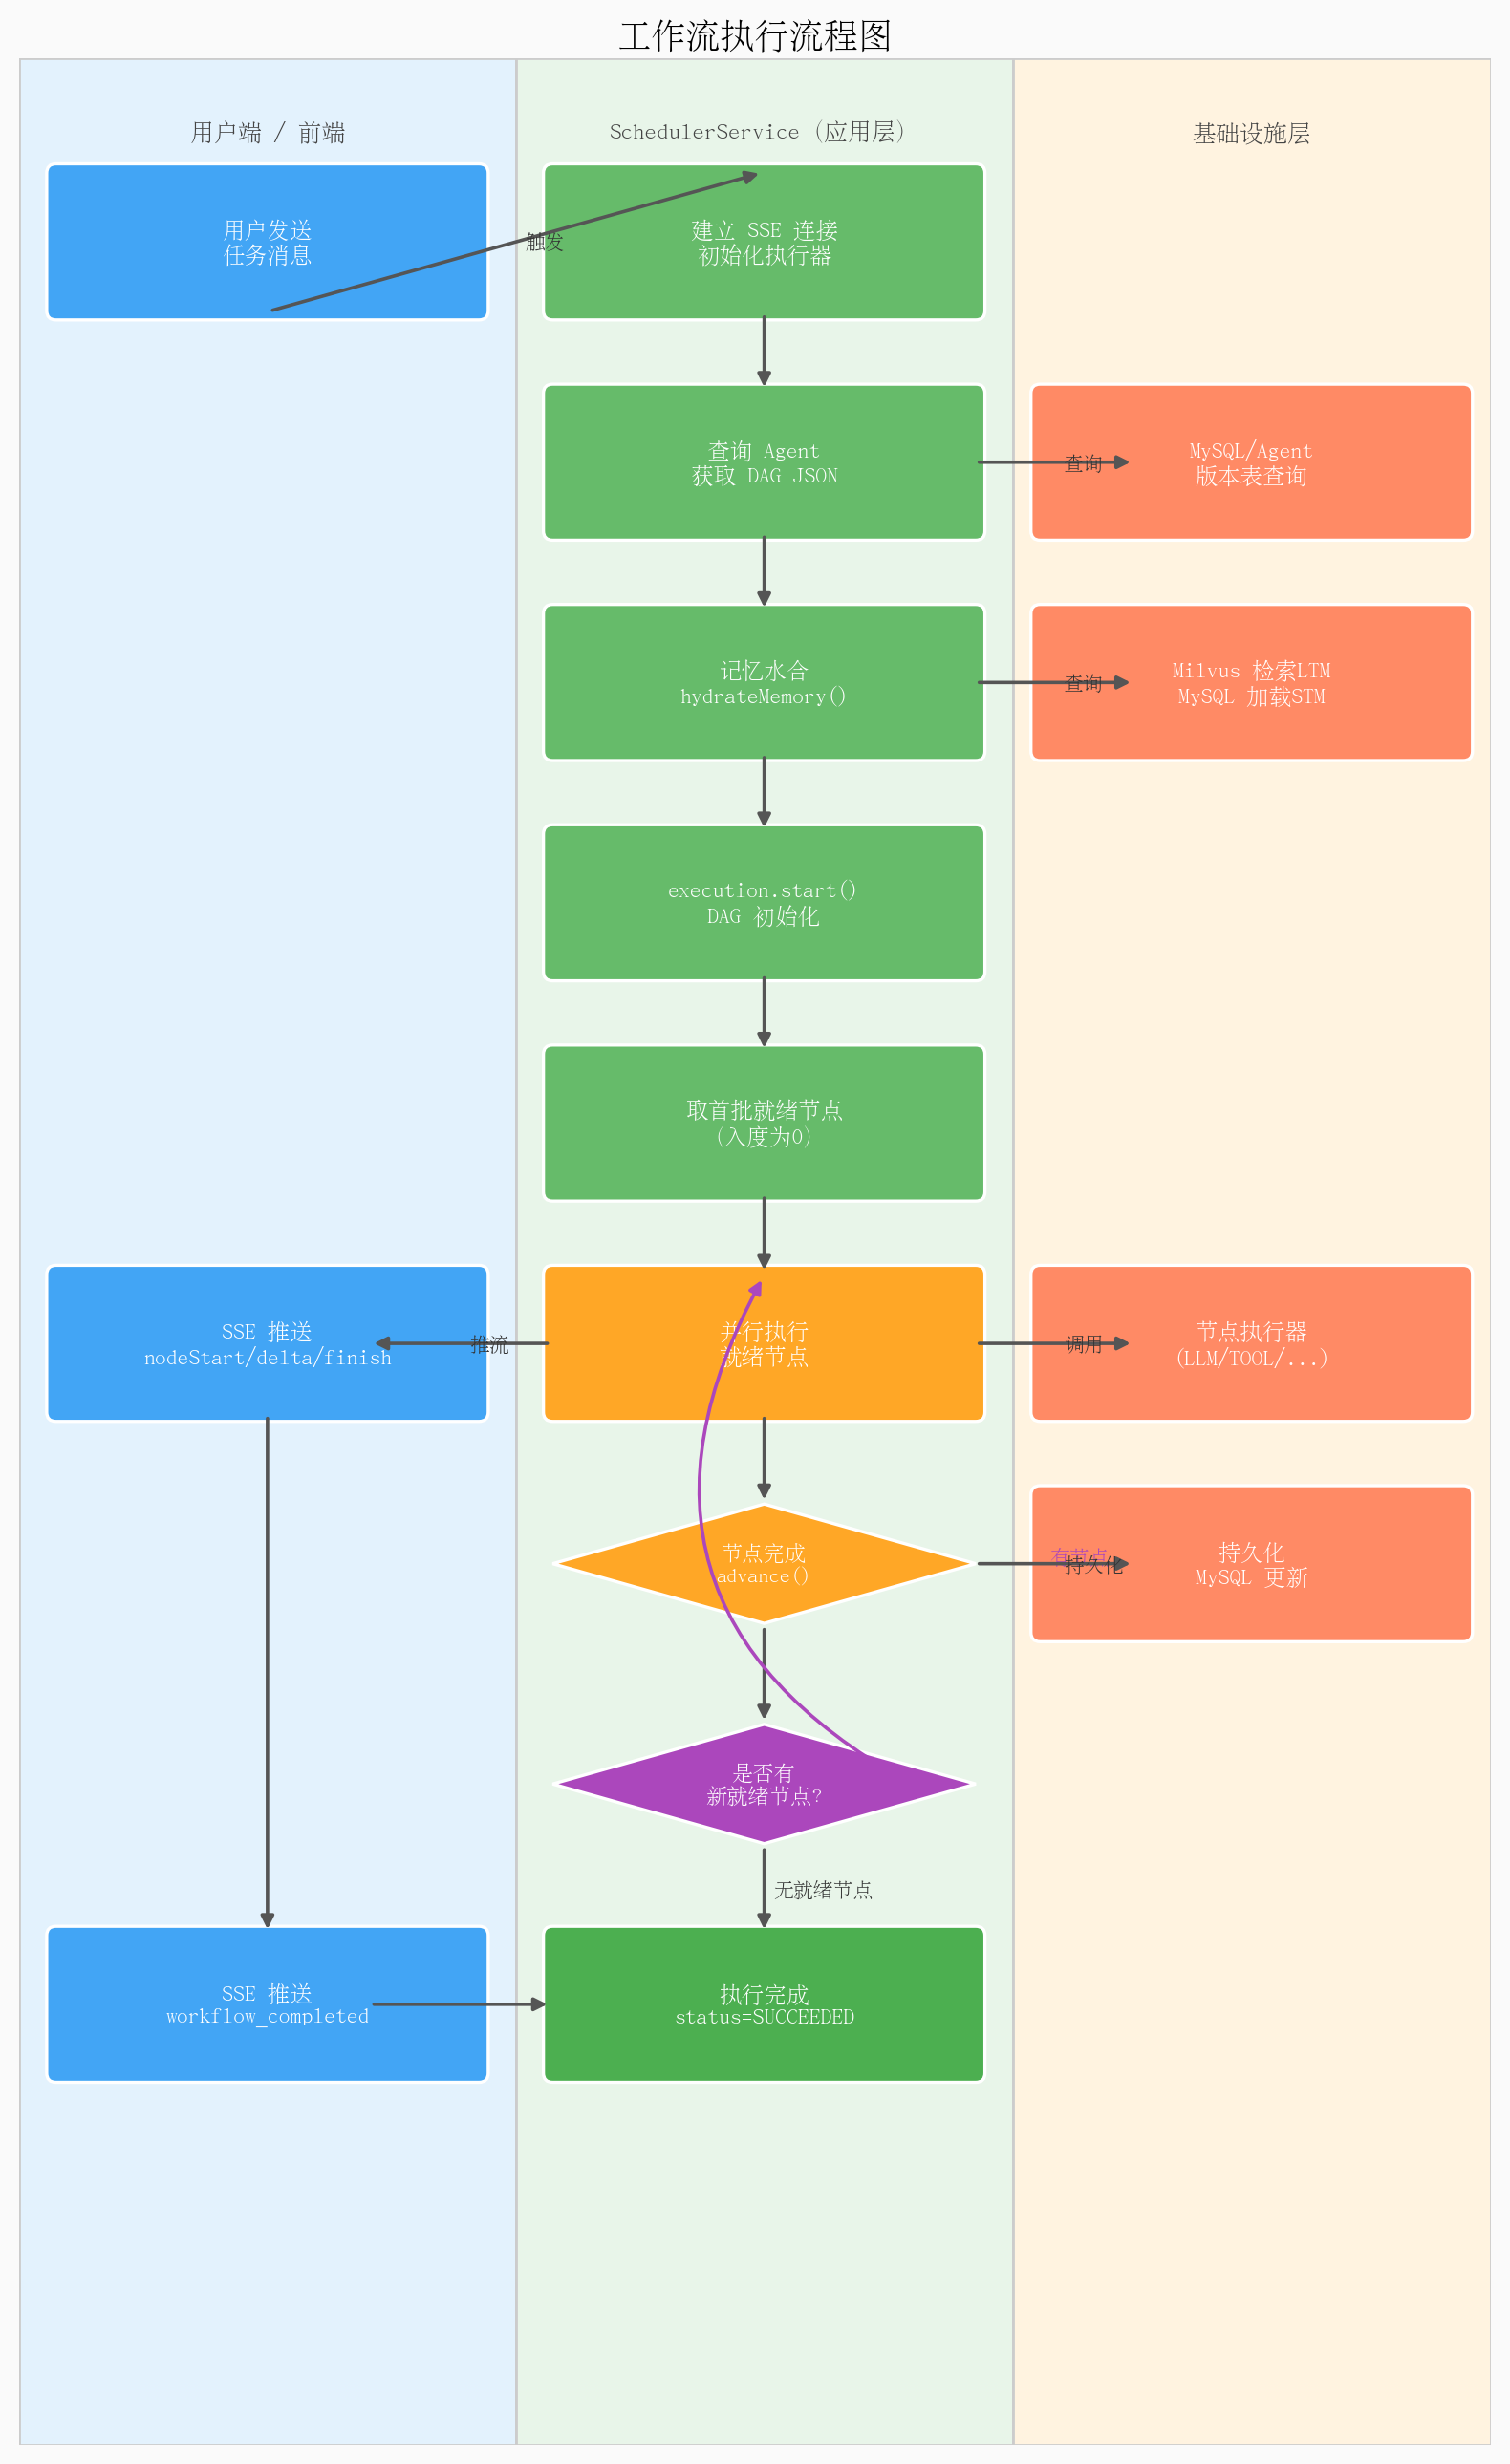
\includegraphics[width=0.68\textwidth]{figures/fig_exec_flow.png}
  \caption{工作流执行流程图}
  \label{fig:exec_flow}
\end{figure}

用户在前端对话界面输入消息后，前端建立 SSE 连接并调用工作流启动接口，
系统首先从向量数据库检索与用户输入语义相关的知识片段，
再从会话存储中加载最近的对话历史，
将两者注入执行上下文后调用 \texttt{execution.start(inputs)} 初始化 DAG。
调度器依次取出就绪节点（入度为 0 的节点）并发执行，
每个节点完成后调用 \texttt{advance()} 推进状态，计算下一批就绪节点，
直至所有节点完成，整体状态更新为 \texttt{SUCCEEDED}。

\subsubsection{（3）人工检查点审批}

表~\ref{tab:uc_review}~为人工审批用例的需求说明表。

\begin{table}[H]
  \centering
  \caption{人工检查点审批用例需求表}
  \label{tab:uc_review}
  \begin{tabular}{|p{3cm}|p{10cm}|}
    \hline
    \textbf{用例标识} & UC-03 人工检查点审批 \\
    \hline
    \textbf{功能描述} & 工作流执行到配置了人工检查点的节点时自动暂停，审批人查看并决策后工作流继续运行 \\
    \hline
    \textbf{使用人员} & 业务人员 / 系统管理员 \\
    \hline
    \textbf{前置条件} & 工作流执行状态为 PAUSED\_FOR\_REVIEW，存在待审批记录 \\
    \hline
    \textbf{输入（通过）} & executionId、nodeId、expectedVersion、可选的 edits（修改内容）、comment \\
    \hline
    \textbf{输入（拒绝）} & executionId、nodeId、expectedVersion、reason（拒绝原因） \\
    \hline
    \textbf{系统响应} & 通过乐观锁校验版本，合并编辑内容，写审批记录，更新执行状态 \\
    \hline
    \textbf{输出（通过）} & 执行恢复（RUNNING），SSE 推送 workflow\_resumed，后续节点继续调度 \\
    \hline
    \textbf{输出（拒绝）} & 执行终止（FAILED），SSE 推送 workflow\_rejected，写拒绝审批记录 \\
    \hline
    \textbf{操作序列} & 执行暂停后前端展示审批面板，审批人决策后系统更新状态并通过 SSE 通知前端 \\
    \hline
    \textbf{异常} & 并发审批（version 不匹配）→ 返回 409 Conflict；节点不匹配 → 返回 400 \\
    \hline
  \end{tabular}
\end{table}

图~\ref{fig:review_flow}~展示了人工检查点的完整流程。

\begin{figure}[H]
  \centering
  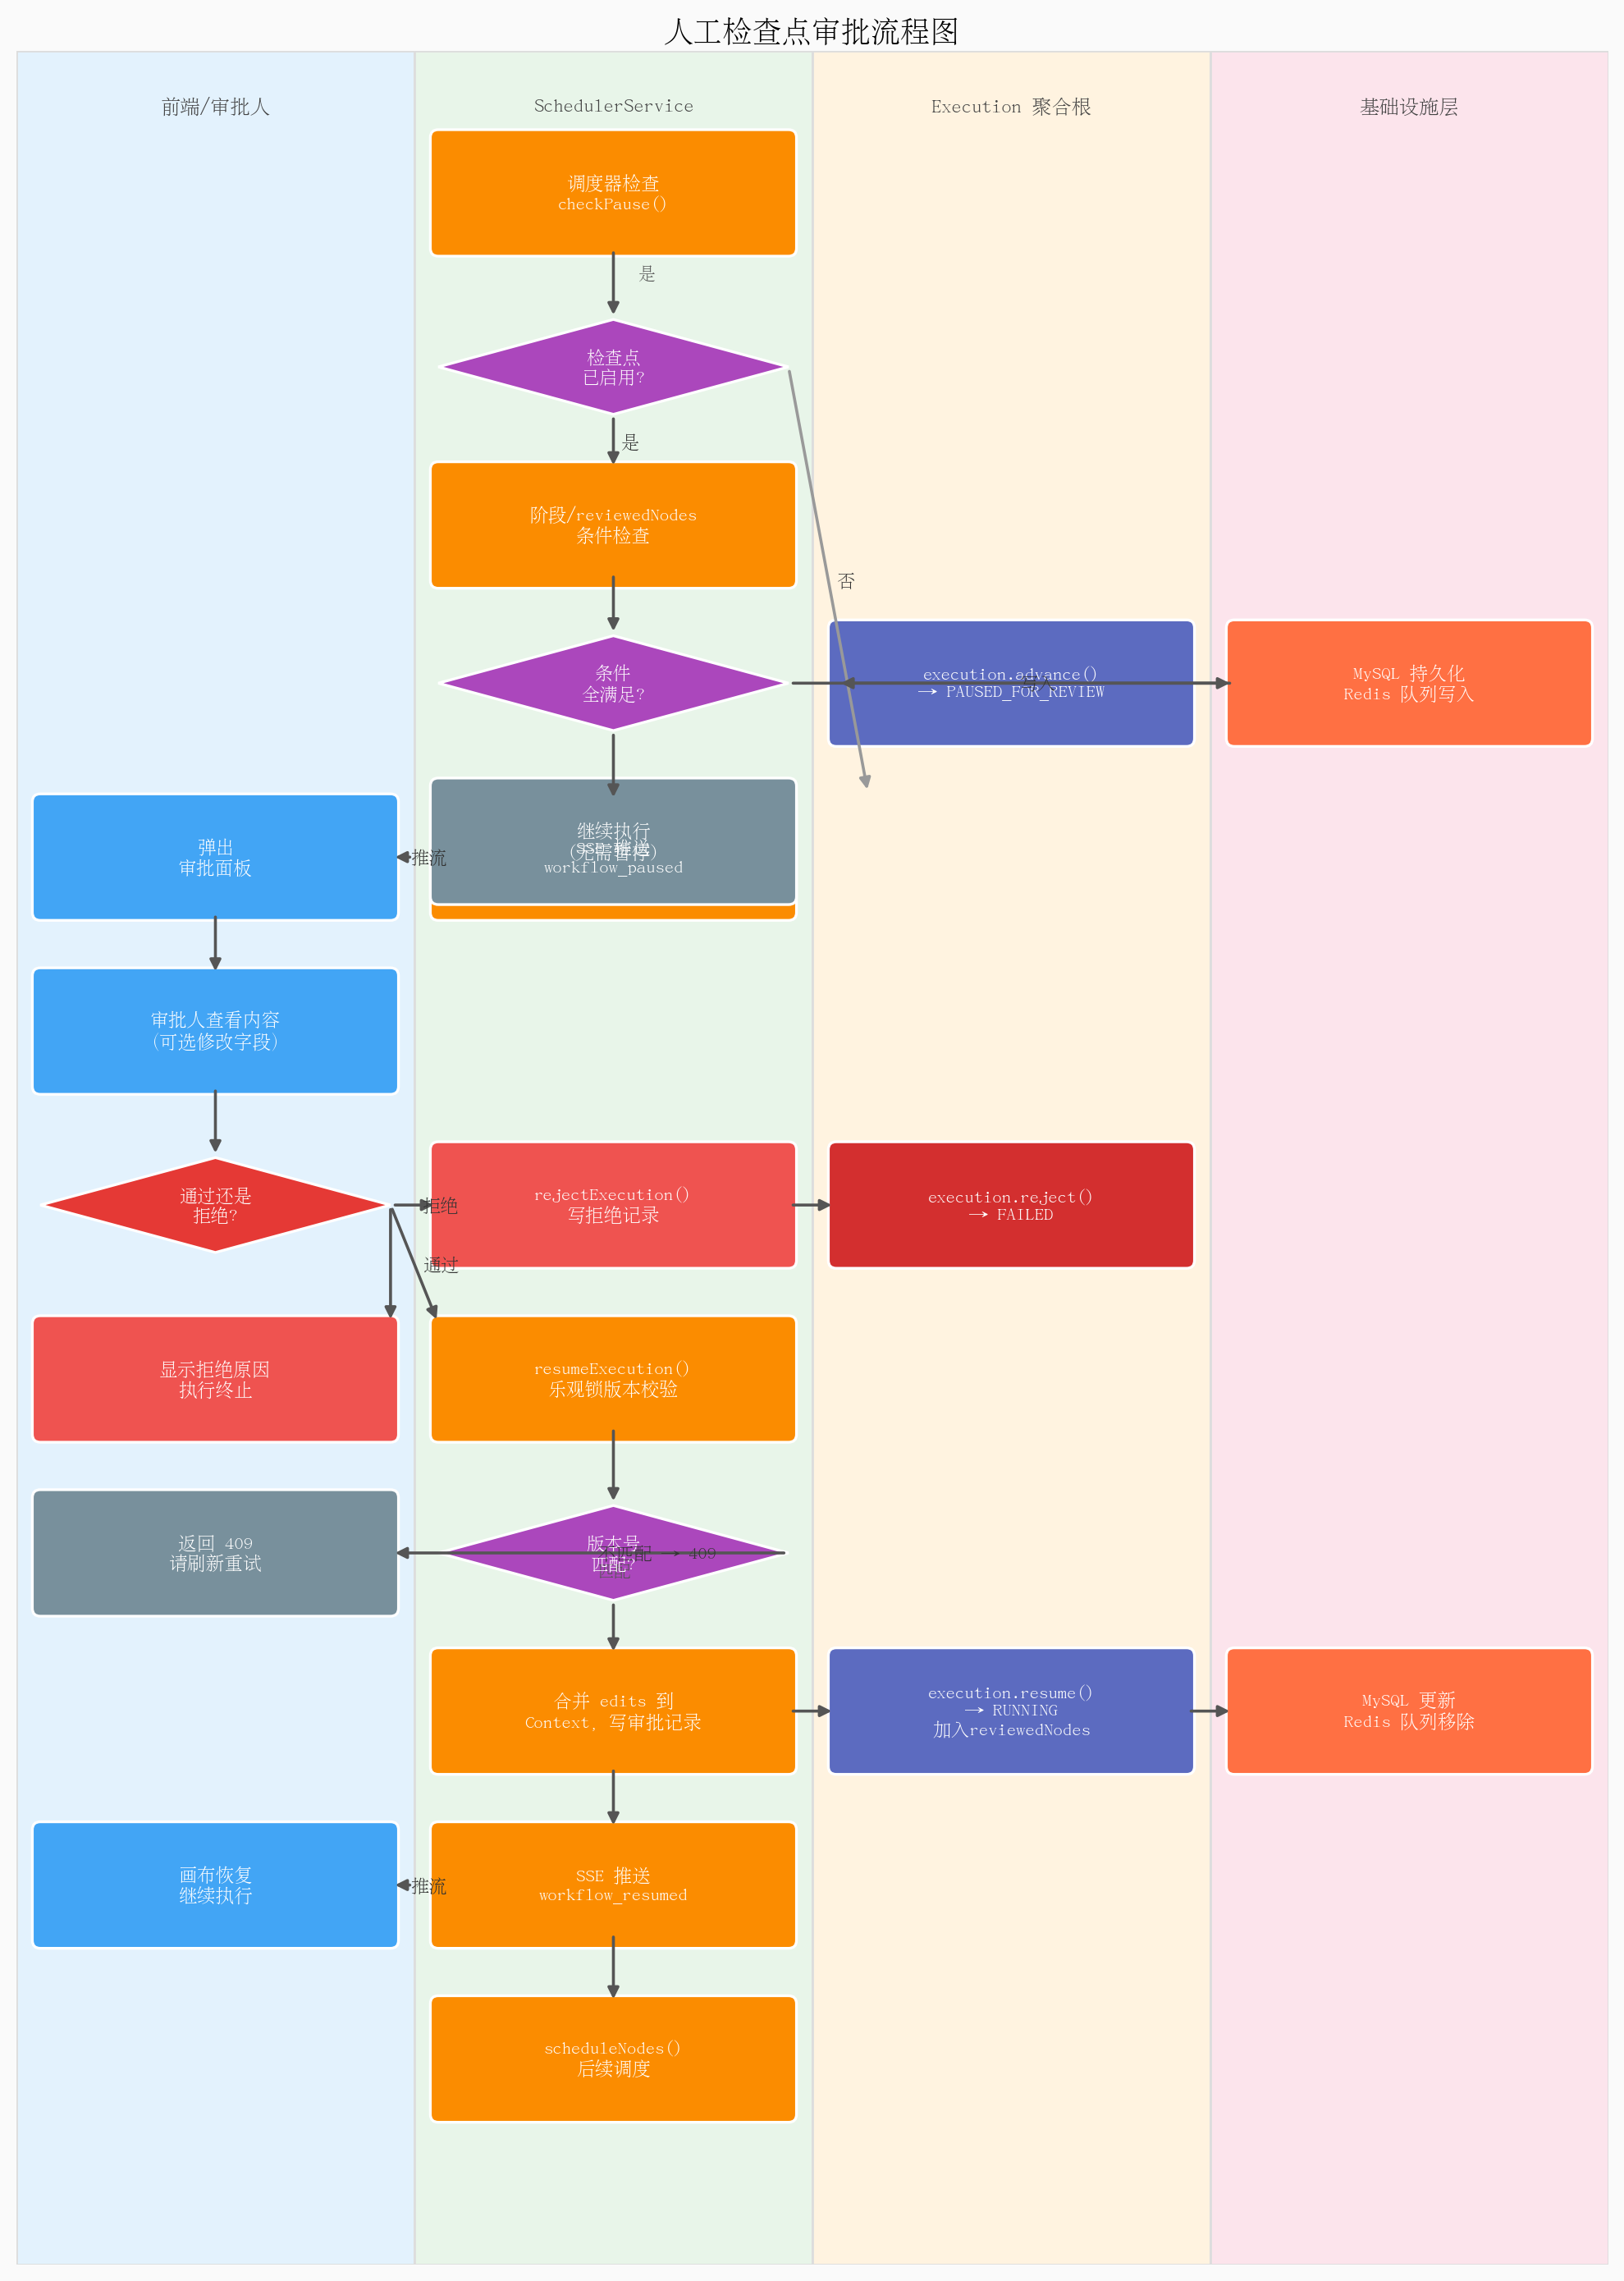
\includegraphics[width=0.72\textwidth]{figures/fig_review_flow.png}
  \caption{人工检查点审批流程图}
  \label{fig:review_flow}
\end{figure}

当执行到配置了检查点的节点时，系统通过 SSE 向前端推送 \texttt{workflow\_paused} 事件，
前端弹出审批面板，展示当前节点的输入（\texttt{BEFORE\_EXECUTION}）
或输出（\texttt{AFTER\_EXECUTION}）内容。
审批人检查内容后，若认为结果需要修正，可直接在面板中编辑字段值；
点击"通过"后，前端携带 \texttt{expectedVersion}（乐观锁）和修改内容提交，
服务端校验版本一致性，合并编辑内容到上下文，写入审批记录，之后恢复工作流执行。
若审批人点击"拒绝"，则工作流立即终止，审批记录中写入拒绝原因。

\subsubsection{（4）知识库检索增强}

表~\ref{tab:uc_knowledge}~为知识库检索增强用例的需求说明表。

\begin{table}[H]
  \centering
  \caption{知识库检索增强用例需求表}
  \label{tab:uc_knowledge}
  \begin{tabular}{|p{3cm}|p{10cm}|}
    \hline
    \textbf{用例标识} & UC-04 知识库检索增强 \\
    \hline
    \textbf{功能描述} & 用户上传文档形成知识库，工作流在运行时根据查询语义召回相关片段增强模型上下文 \\
    \hline
    \textbf{使用人员} & 业务人员 / 系统管理员 / 系统（自动检索） \\
    \hline
    \textbf{前置条件} & 知识文档已上传并完成向量化入库，Milvus Collection 已就绪 \\
    \hline
    \textbf{输入} & 文档文件、分块配置、用户查询语句 \\
    \hline
    \textbf{系统响应} & 解析文档、文本分块、调用嵌入模型写入向量库，并在运行时完成 Top-K 语义检索 \\
    \hline
    \textbf{输出} & 检索到的相关片段写入上下文，供后续 LLM 节点拼接使用 \\
    \hline
    \textbf{操作序列} & 用户上传文档后系统异步处理并向量化，运行时检索相关片段增强模型输入 \\
    \hline
    \textbf{异常} & Milvus 不可达 → 记录异常日志并降级；文档解析失败 → 文档状态标记 FAILED \\
    \hline
  \end{tabular}
\end{table}

\subsubsection{（5）用户注册与登录}

表~\ref{tab:uc_auth}~为用户注册与登录用例的需求说明表。

\begin{table}[H]
  \centering
  \caption{用户注册与登录用例需求表}
  \label{tab:uc_auth}
  \begin{tabular}{|p{3cm}|p{10cm}|}
    \hline
    \textbf{用例标识} & UC-05 用户注册与登录 \\
    \hline
    \textbf{功能描述} & 用户通过邮箱验证码完成注册，并在登录成功后获取访问令牌使用系统功能 \\
    \hline
    \textbf{使用人员} & 普通用户 / 系统管理员 \\
    \hline
    \textbf{前置条件} & 邮件服务正常，验证码缓存服务可用 \\
    \hline
    \textbf{输入} & 邮箱、验证码、密码、用户名、登录 IP \\
    \hline
    \textbf{系统响应} & 校验验证码、密码强度与账号唯一性，完成密码加密和用户身份校验 \\
    \hline
    \textbf{输出} & 注册成功返回用户信息；登录成功返回访问令牌；失败时返回错误原因 \\
    \hline
    \textbf{操作序列} & 用户获取邮箱验证码并提交注册信息，登录成功后系统签发 JWT 访问令牌 \\
    \hline
    \textbf{异常} & 验证码错误或过期 → 注册失败；密码错误次数过多 → 登录受限；邮箱重复注册 → 拒绝创建 \\
    \hline
  \end{tabular}
\end{table}

\section{非功能需求}

\subsection{性能需求}

\begin{itemize}
  \item 核心非流式接口应具备良好的实时响应能力，能够满足管理与审批场景下的交互要求
  \item SSE 执行状态推送端到端延迟应控制在秒级以内，保证前端画布和日志实时更新
  \item 调度器从节点就绪到触发执行的延迟应足够低，能够支持多节点顺畅推进
\end{itemize}

\subsection{可靠性需求}

\begin{itemize}
  \item 工作流执行状态持久化到 MySQL，历史记录可查
  \item Redis 维护待审批队列和分布式锁，乐观锁保障并发安全
  \item 文档处理状态、审批记录和执行日志均需具备可恢复、可追溯能力
\end{itemize}

\subsection{可扩展性需求}

\begin{itemize}
  \item 节点执行器采用策略模式，新节点类型只需实现 \texttt{NodeExecutorStrategy} 接口
  \item 大模型接口通过 Spring AI 统一适配，支持多厂商模型切换
  \item 知识分块策略、向量存储和邮件服务等基础能力应可替换扩展
\end{itemize}

\subsection{安全性需求}

\begin{itemize}
  \item 所有 REST API 接口通过 JWT Token 鉴权
  \item 密码需以加密哈希形式存储，禁止明文保存
  \item 验证码发送和登录失败均需具备频率限制
  \item 审批操作记录操作人（reviewerId）并持久化，满足审计合规要求
\end{itemize}

\section{本章小结}

本章围绕三类用户角色系统梳理了功能需求，
并将系统能力统一收束为 Agent 管理与可视化编排、工作流调度执行、
人工审核与恢复机制、知识库与检索增强、用户认证与系统安全支撑五个模块。
通过五个关键用例的需求表格与流程描述，明确了系统的主要交互链路，
并从性能、可靠性、可扩展性和安全性四个维度给出了非功能需求，
为后续系统设计与实现奠定了需求基础。
   %% 第2章 系统需求分析
%% 第3章 AI Agent 智能体编排系统概要设计

\chapter{AI Agent 智能体编排系统概要设计}

\section{系统结构设计}

系统采用\textbf{领域驱动设计（DDD）的分层架构}和前后端分离的部署模式，
后端分为接口层、应用层、领域层、基础设施层四个 Maven 子模块，
前端基于 React + TypeScript 实现。系统整体结构如图~\ref{fig:sys_struct}~所示。

\begin{figure}[H]
  \centering
  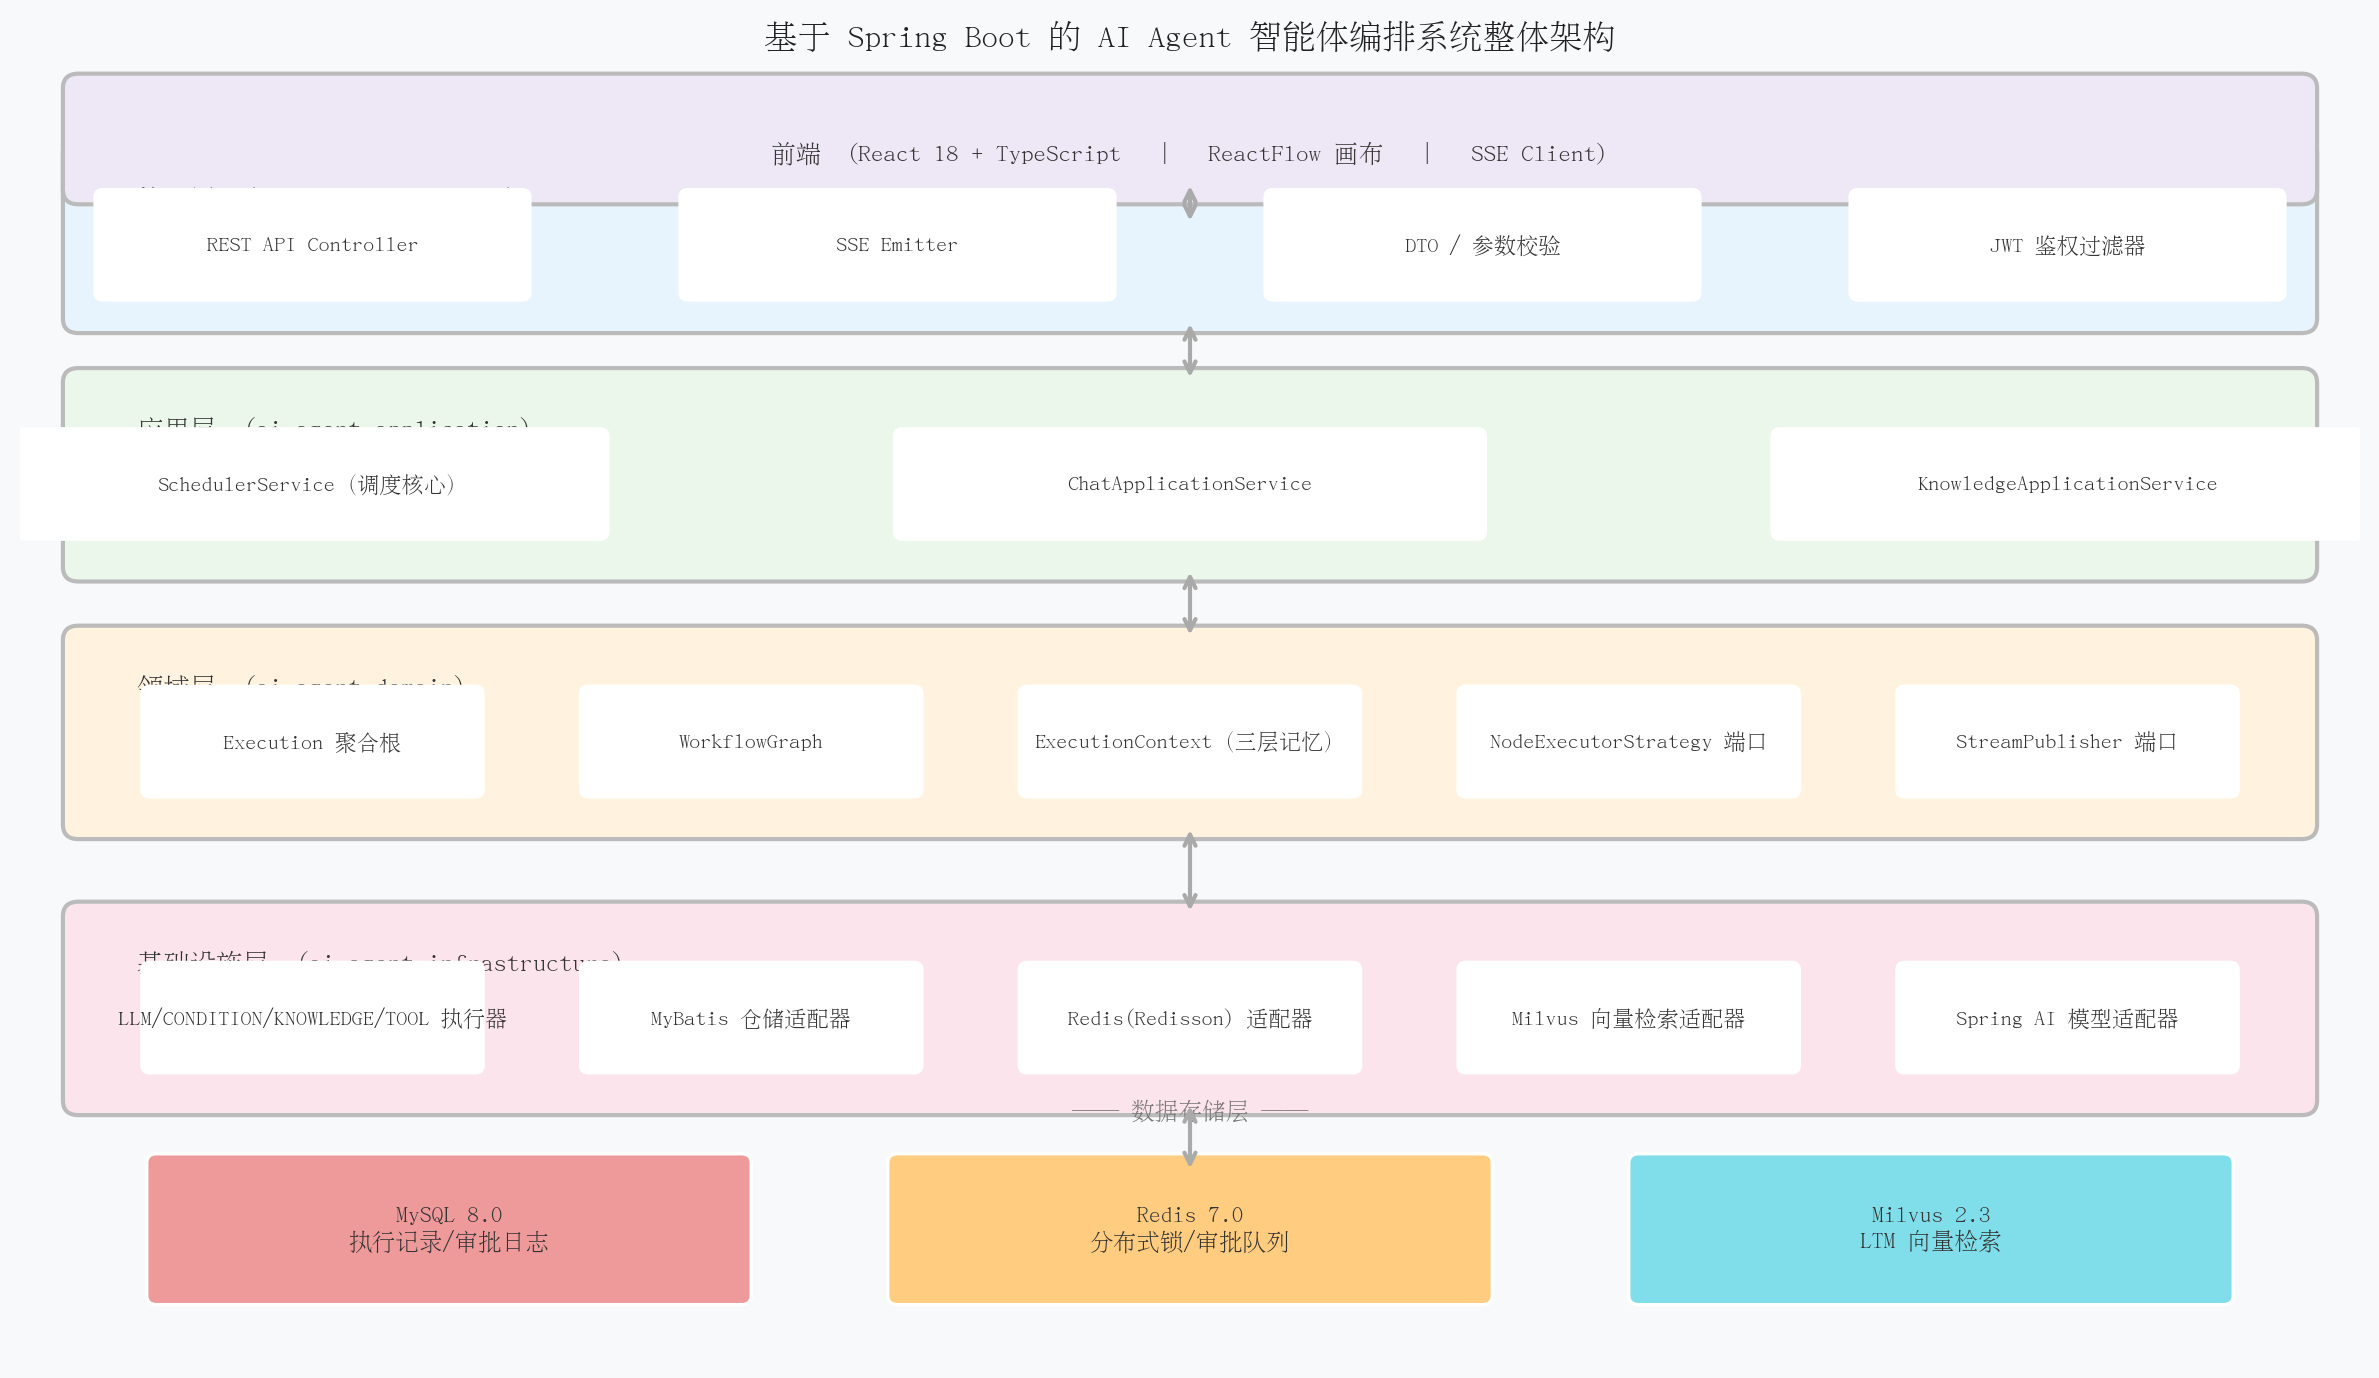
\includegraphics[width=0.95\textwidth]{figures/fig_arch.png}
  \caption{系统整体结构图}
  \label{fig:sys_struct}
\end{figure}

各层的技术组成和核心职责如下：

\textbf{接口层（ai-agent-interfaces）：}
提供 RESTful API 控制器（Controller），负责处理 HTTP 请求、参数校验、
DTO 与领域对象的转换，以及 SSE 连接的建立与维护。
用户注册、登录、知识库管理、审批接口和工作流启动接口均在此层对外暴露。

\textbf{应用层（ai-agent-application）：}
包含 Agent 管理服务、工作流调度服务、知识应用服务和用户应用服务等。
该层负责跨聚合编排，例如协调 Agent 查询、工作流 DAG 解析、知识检索增强、
审批恢复与异步文档处理等，但不承载具体领域规则本身。

\textbf{领域层（ai-agent-domain）：}
系统业务逻辑的核心，包含 \texttt{Execution} 聚合根（DAG 状态流转）、
\texttt{WorkflowGraph}（图结构）、\texttt{KnowledgeDocument}、\texttt{User} 等核心领域对象，
以及向量检索、文件存储、文本切分、邮件服务等端口接口。
领域层保持纯净，不依赖任何框架或外部库。

\textbf{基础设施层（ai-agent-infrastructure）：}
实现领域层定义的端口接口，包括节点执行器策略（LLM/CONDITION/KNOWLEDGE/TOOL/START/END）、
MySQL 仓储适配器、Redis 客户端、Milvus 向量存储适配器、MinIO 文件存储适配器、
邮件发送实现以及 Spring AI 模型适配器。

前端（ai-agent-forward）基于 React + TypeScript 实现，
包含 Agent 列表与画布编排页、对话执行页、人工审批页、知识库页和登录注册页等功能页面。

\section{系统功能设计}

根据需求分析，系统围绕五个核心模块展开设计，功能结构如图~\ref{fig:func_struct}~所示。

\begin{figure}[H]
  \centering
  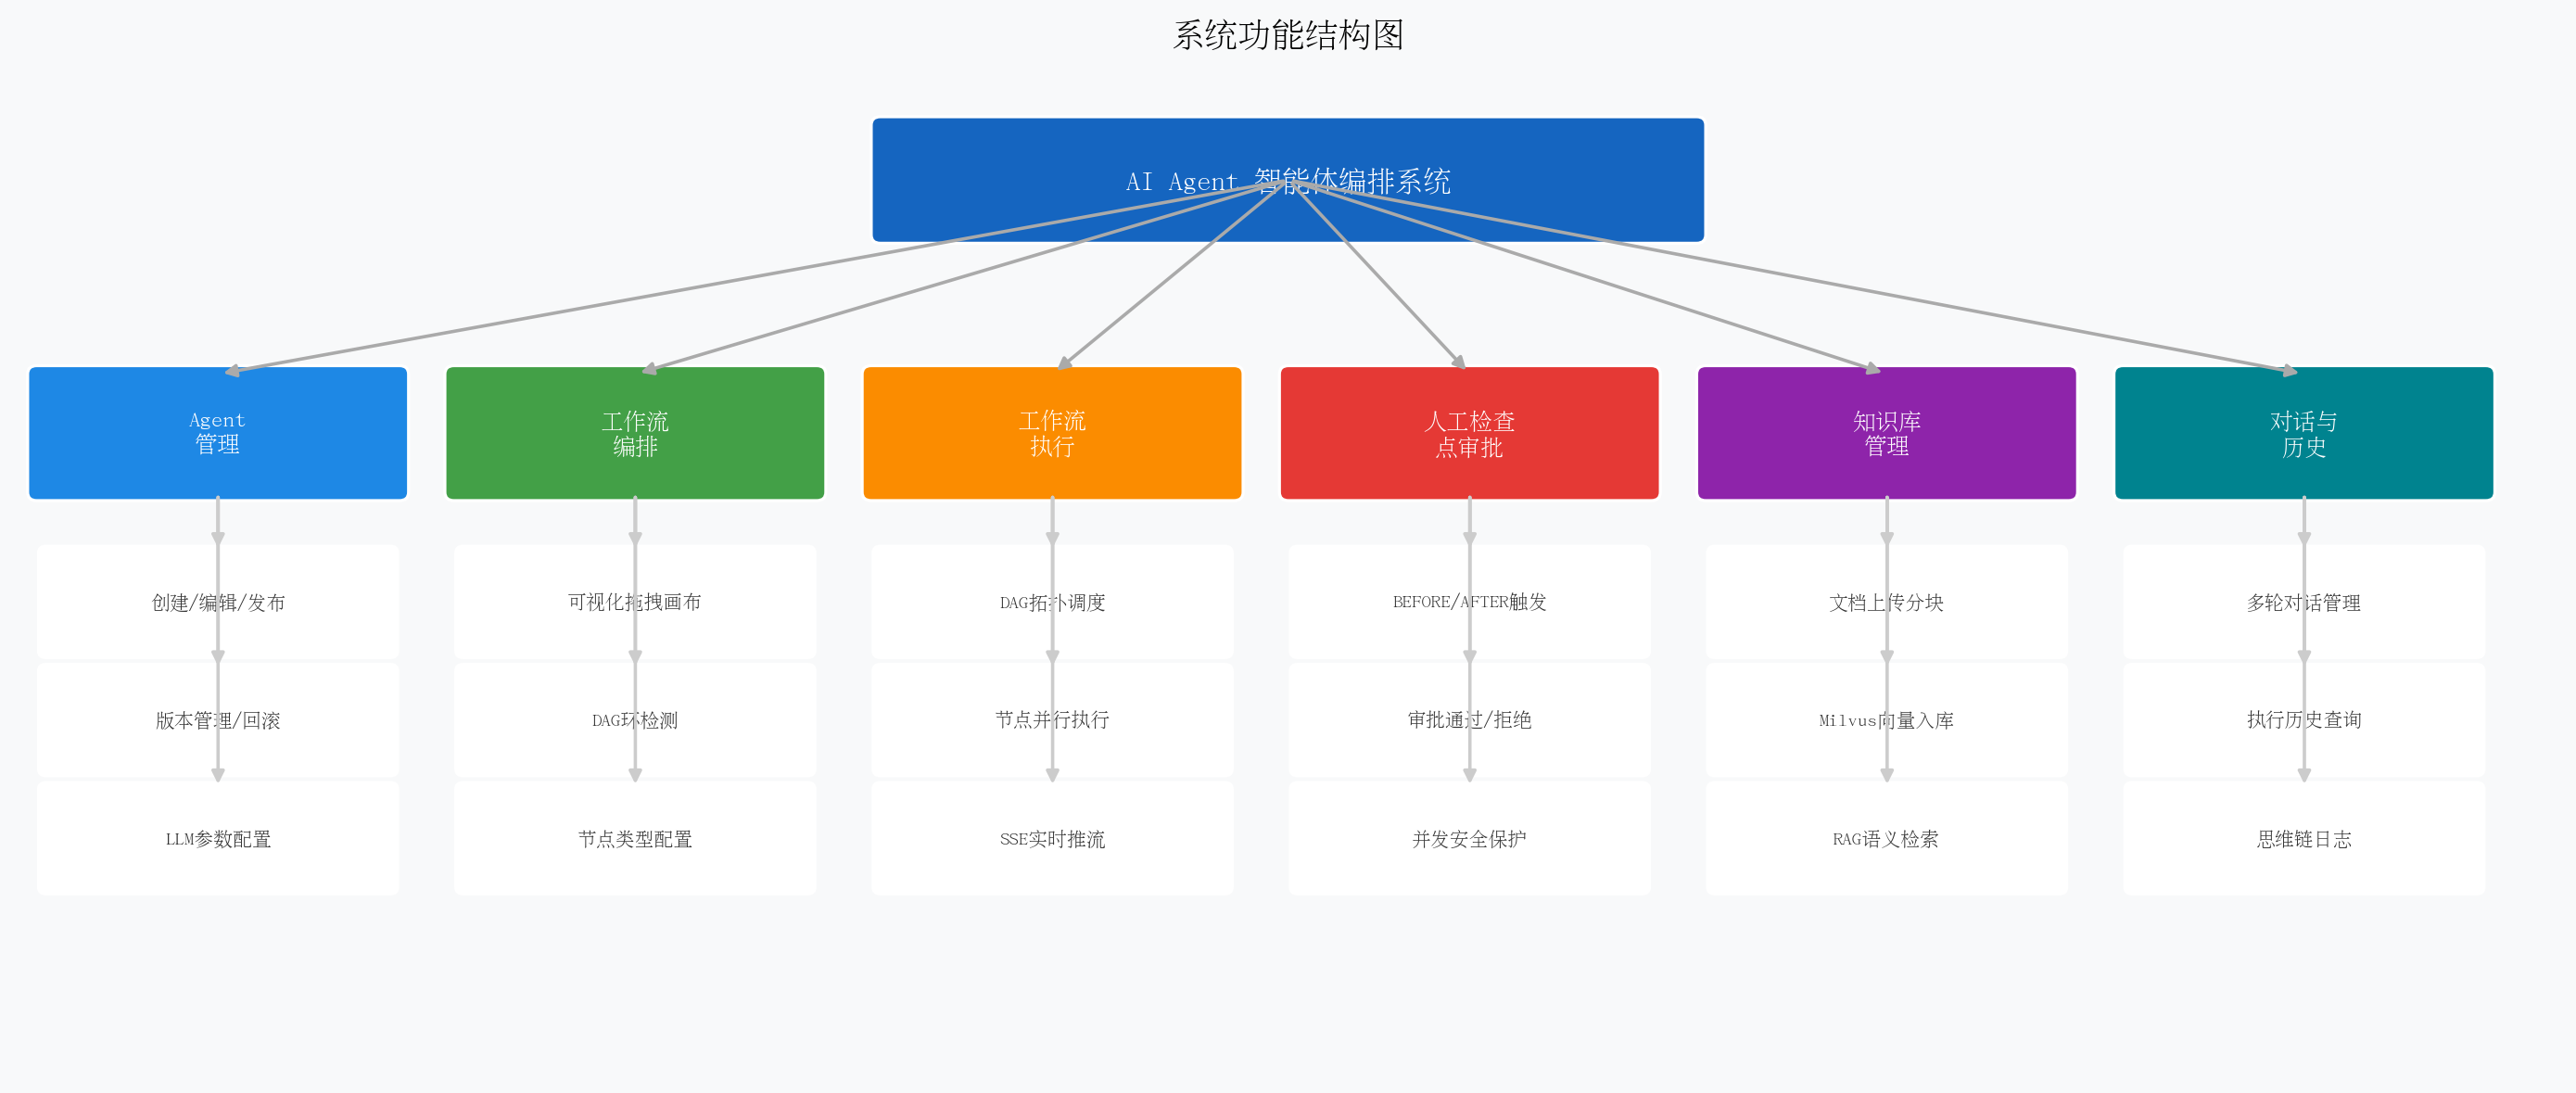
\includegraphics[width=0.98\textwidth]{figures/fig_func.png}
  \caption{系统功能结构图}
  \label{fig:func_struct}
\end{figure}

\subsection{Agent 管理与可视化编排模块}

该模块负责 Agent 的生命周期管理与可视化流程定义。
后端通过 Agent 应用服务实现创建、编辑、发布、版本查询与回滚，
每个 Agent 对应一份以 \texttt{graphJson} 形式存储的工作流定义。
前端通过 ReactFlow 画布提供拖拽式编排界面，支持节点创建、删除、参数配置和边连接，
并将画布状态统一序列化为图结构 JSON。

在发布流程中，系统会将当前草稿快照写入 \texttt{agent\_version} 表，
并更新 Agent 的已发布版本号，保证编辑中的草稿和线上执行版本相互隔离。
通过这一设计，Agent 管理模块既承担配置入口，又为运行时调度提供标准化图定义来源。

\subsection{工作流调度执行模块}

工作流执行模块以 \texttt{SchedulerService} 与 \texttt{Execution} 聚合根的协作为核心。
系统在执行开始时读取 Agent 的图定义，将 \texttt{graphJson} 反序列化为 \texttt{WorkflowGraph}，
随后初始化执行上下文、节点状态和就绪队列。

执行引擎基于 DAG 拓扑排序和事件驱动调度，
支持无依赖节点并行执行、条件分支、路径剪枝和执行状态推进。
整个执行过程通过 SSE 持续向前端推送节点启动、完成、错误和暂停恢复等事件。

执行状态机如图~\ref{fig:state_machine}~所示。

\begin{figure}[H]
  \centering
  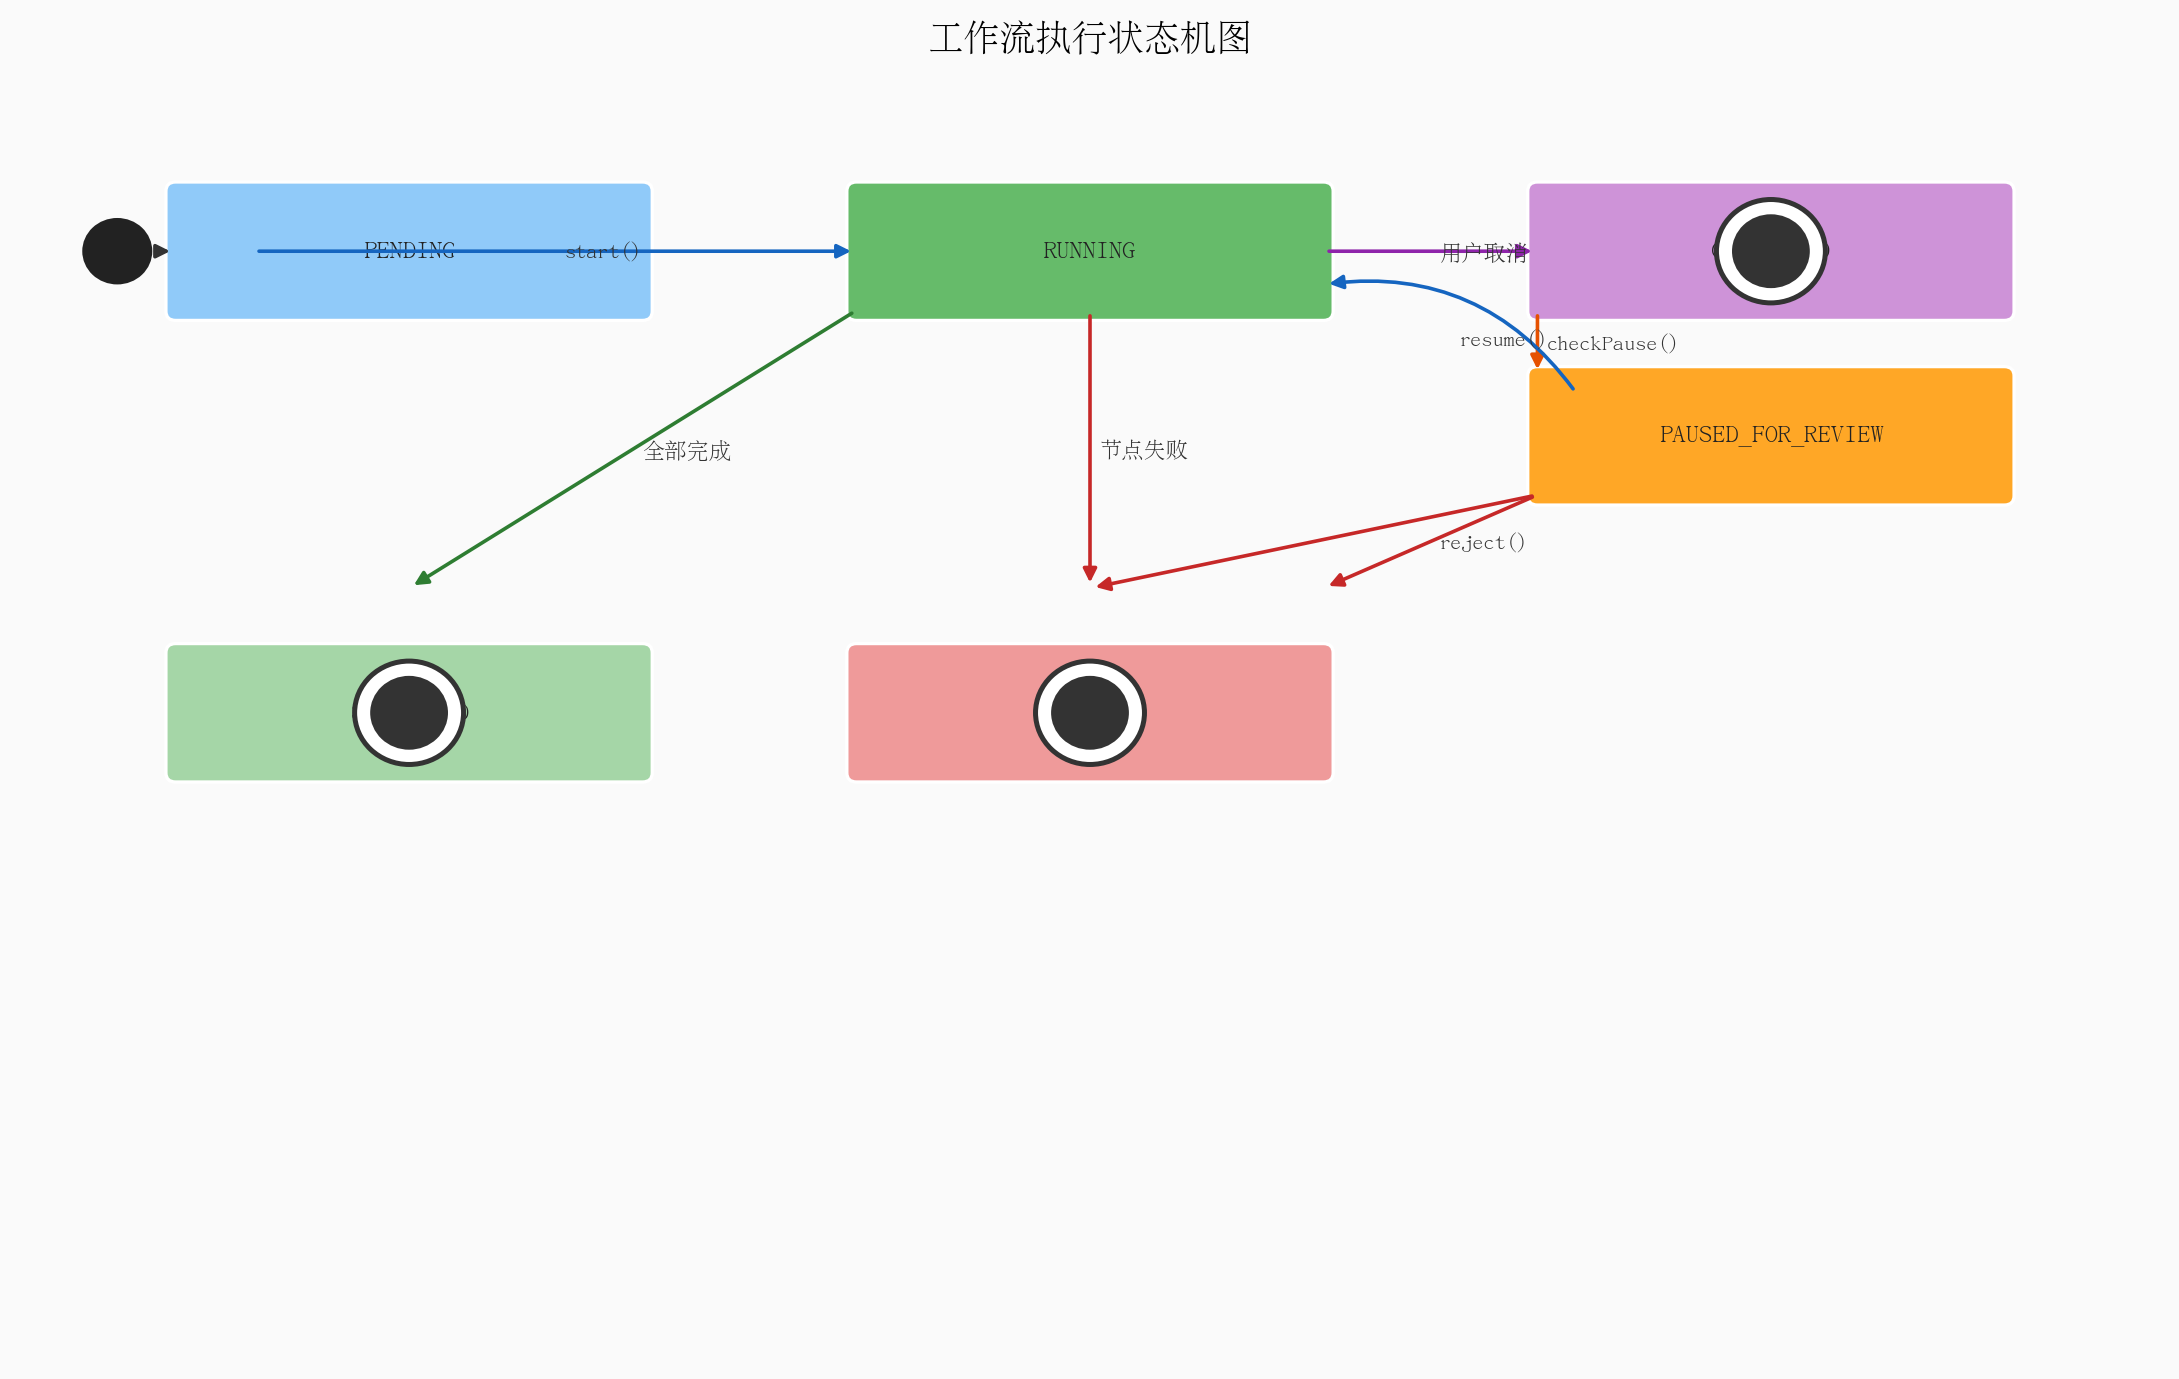
\includegraphics[width=0.88\textwidth]{figures/fig_state.png}
  \caption{工作流执行状态机}
  \label{fig:state_machine}
\end{figure}

\begin{table}[H]
  \centering
  \caption{执行状态转换说明}
  \begin{tabular}{lll}
    \toprule
    \textbf{源状态} & \textbf{目标状态} & \textbf{触发条件} \\
    \midrule
    PENDING & RUNNING & \texttt{start()} 调用成功，DAG 初始化 \\
    RUNNING & SUCCEEDED & 所有节点均完成（SUCCEEDED 或 SKIPPED） \\
    RUNNING & FAILED & 某节点执行失败 \\
    RUNNING & CANCELLED & 用户主动取消 \\
    RUNNING & PAUSED\_FOR\_REVIEW & 检查点触发，执行进入人工审核 \\
    PAUSED\_FOR\_REVIEW & RUNNING & 审批通过，\texttt{resume()} \\
    PAUSED\_FOR\_REVIEW & FAILED & 审批拒绝，\texttt{reject()} \\
    \bottomrule
  \end{tabular}
  \label{tab:state_trans}
\end{table}

\subsection{人工审核与恢复机制模块}

该模块在工作流执行链路中植入“暂停—等待—恢复/终止”的控制能力。
节点可配置人工检查点开关与触发阶段，支持 \texttt{BEFORE\_EXECUTION}
和 \texttt{AFTER\_EXECUTION} 两种模式。

设计上，系统采用 Redis 维护待审批队列，并为每个执行实例配置分布式锁；
审批人通过审批列表接口查看待处理任务，进入详情后可查看当前节点上下文、
修改中间结果并提交通过或拒绝操作。
恢复或拒绝请求均以执行版本号作为乐观锁条件，
从而防止多用户并发审批导致的状态覆盖问题。

\subsection{知识库与检索增强模块}

该模块用于为工作流中的知识节点和 LLM 节点提供外部知识支撑。
从设计上看，知识链路由数据集管理、文档管理、异步处理和语义检索四部分组成。

用户上传文档后，系统先将原始文件存入 MinIO，
再由异步处理器完成文档解析、文本分块与向量化入库。
向量数据与原始文档元信息通过 \texttt{document\_id}、\texttt{dataset\_id}、\texttt{agent\_id}
等字段建立关联，便于后续删除、筛选与语义搜索。

运行时，当知识节点或检索接口收到查询请求时，系统将查询语句向量化，
在 Milvus 中执行 Top-K 语义搜索，并将召回片段返回给后续节点作为上下文增强信息。
这一设计使知识接入链路与工作流运行链路形成完整闭环。

\subsection{用户认证与系统安全支撑模块}

该模块为整个平台提供统一的身份识别、访问控制与安全约束能力。
系统支持邮箱注册、登录、找回密码和 JWT 令牌认证，
其中验证码发送、密码强度校验、密码哈希存储与登录失败限制均在认证领域服务中实现。

认证成功后，接口层在请求上下文中解析用户身份，
业务模块据此执行 Agent 所有权校验、知识库访问控制、审批操作记录等逻辑。
因此，用户认证与系统安全并不是孤立模块，而是贯穿其他四个业务模块的基础支撑层。

\section{核心数据流设计}

为体现五个模块之间的衔接关系，系统在设计上形成了如下三条关键数据流。

\subsection{Agent 编排到运行时执行的数据流}

用户在前端画布完成 Agent 编排后，画布中的节点和边会被序列化为 \texttt{graphJson}。
当用户点击保存时，后端执行图结构校验并将其保存为草稿；
点击发布后，系统生成版本快照并固化为可执行版本。
运行时，调度器根据 Agent ID 与版本号读取对应的图定义，
再将 JSON 反序列化为 \texttt{WorkflowGraph}，作为 \texttt{Execution} 聚合根的输入。

\subsection{知识接入到检索增强的数据流}

用户上传文档后，接口层将文件流和分块配置传递给知识应用服务；
应用服务先进行文件校验并上传到 MinIO，再创建文档记录并触发异步处理器。
异步处理器下载原始文件，解析为文本段落，调用文本切分器生成多个文本块，
随后通过向量存储接口将其写入 Milvus。
执行期收到查询时，系统以相同的语义向量检索方式召回相关片段，
再将其注入工作流上下文供后续节点使用。

\subsection{认证安全到业务访问控制的数据流}

用户注册或登录成功后，系统签发 JWT 令牌，前端在后续请求中统一携带。
接口层解析令牌并写入当前用户上下文，应用服务据此进行资源所有权校验。
例如 Agent 更新必须校验 Agent 是否属于当前用户，
知识文档上传必须校验数据集归属，人工审批记录必须保存当前审批人 ID。
这一数据流保证了平台各模块均运行在统一的认证与授权边界内。

\section{数据库设计}

系统采用 MySQL 8.0 存储业务数据，核心数据表清单如表~\ref{tab:db_tables}~所示。

\begin{table}[H]
  \centering
  \caption{核心数据表清单}
  \label{tab:db_tables}
  \begin{tabular}{lll}
    \toprule
    \textbf{表名} & \textbf{所属模块} & \textbf{用途} \\
    \midrule
    \texttt{agent} & Agent 管理 & Agent 基本信息与草稿图定义 \\
    \texttt{agent\_version} & Agent 管理 & Agent 版本快照（含 graphJson） \\
    \texttt{workflow\_execution} & 工作流执行 & 执行记录（状态/暂停节点/版本号/上下文） \\
    \texttt{workflow\_execution\_node} & 工作流执行 & 节点执行日志（输入/输出/耗时） \\
    \texttt{workflow\_human\_review\_record} & 人工审核 & 审批记录（审批人/决策/修改内容/原因） \\
    \texttt{knowledge\_dataset} & 知识库 & 知识数据集基本信息 \\
    \texttt{knowledge\_document} & 知识库 & 文档记录、处理状态和分块配置 \\
    \texttt{user} & 用户认证 & 用户账户信息与密码哈希 \\
    \texttt{chat\_conversation} & 对话 & 会话记录 \\
    \texttt{chat\_message} & 对话 & 消息记录与短期上下文 \\
    \bottomrule
  \end{tabular}
\end{table}

表~\ref{tab:execution_schema}~列出了 \texttt{workflow\_execution} 表的关键字段设计，
该表是工作流执行状态的核心持久化存储。

\begin{table}[H]
  \centering
  \caption{workflow\_execution 关键字段设计}
  \label{tab:execution_schema}
  \begin{tabular}{llll}
    \toprule
    \textbf{字段名} & \textbf{类型} & \textbf{说明} & \textbf{备注} \\
    \midrule
    execution\_id & VARCHAR & 执行唯一标识 & 主键，UUID \\
    agent\_id & BIGINT & 所属 Agent & 外键 \\
    user\_id & BIGINT & 触发用户 & 外键 \\
    status & VARCHAR & 执行状态枚举 & 见状态机表 \\
    paused\_node\_id & VARCHAR & 当前暂停节点 & 暂停时设置，恢复后清空 \\
    paused\_phase & VARCHAR & 暂停阶段 & BEFORE / AFTER\_EXECUTION \\
    version & INT & 乐观锁版本号 & 每次状态变更自增 \\
    node\_statuses & JSON & 各节点状态 Map & PENDING/RUNNING/SUCCEEDED/FAILED/SKIPPED \\
    context & JSON & 执行上下文快照 & 含 inputs/nodeOutputs/chatHistory/检索结果 \\
    reviewed\_nodes & JSON & 已审批节点集合 & 防止 resume 后重复暂停 \\
    \bottomrule
  \end{tabular}
\end{table}

表~\ref{tab:review_schema}~列出了 \texttt{workflow\_human\_review\_record} 表的关键字段，
该表记录所有人工审批操作，用于事后审计和合规查询。

\begin{table}[H]
  \centering
  \caption{workflow\_human\_review\_record 关键字段设计}
  \label{tab:review_schema}
  \begin{tabular}{llll}
    \toprule
    \textbf{字段名} & \textbf{类型} & \textbf{说明} & \textbf{备注} \\
    \midrule
    id & BIGINT & 主键 & 自增 \\
    execution\_id & VARCHAR & 关联执行 ID & 外键 \\
    node\_id & VARCHAR & 审批节点 ID & 与 DAG 节点一致 \\
    reviewer\_id & BIGINT & 审批人用户 ID & 外键 \\
    decision & VARCHAR & 审批决策 & APPROVE / REJECT \\
    trigger\_phase & VARCHAR & 触发阶段 & BEFORE / AFTER\_EXECUTION \\
    original\_data & JSON & 节点原始输出 & reject 时记录 \\
    modified\_data & JSON & 审批人修改内容 & approve + edits 时记录 \\
    comment & VARCHAR & 审批意见/拒绝原因 & 可为空 \\
    reviewed\_at & DATETIME & 审批时间 & NOT NULL \\
    \bottomrule
  \end{tabular}
\end{table}

表~\ref{tab:knowledge_schema}~列出了知识文档表的关键字段设计。

\begin{table}[H]
  \centering
  \caption{knowledge\_document 关键字段设计}
  \label{tab:knowledge_schema}
  \begin{tabular}{llll}
    \toprule
    \textbf{字段名} & \textbf{类型} & \textbf{说明} & \textbf{备注} \\
    \midrule
    document\_id & VARCHAR & 文档唯一标识 & 主键 \\
    dataset\_id & VARCHAR & 所属数据集 & 外键 \\
    filename & VARCHAR & 原始文件名 & 上传时写入 \\
    file\_url & VARCHAR & 对象存储地址 & MinIO 文件路径 \\
    status & VARCHAR & 处理状态 & PENDING/PROCESSING/COMPLETED/FAILED \\
    total\_chunks\_count & INT & 分块总数 & 处理完成后更新 \\
    chunking\_config & JSON & 分块配置 & 固定分块/语义分块参数 \\
    \bottomrule
  \end{tabular}
\end{table}

\section{技术选型}

表~\ref{tab:tech_stack}~列出了系统各层次的技术选型及选择依据。

\begin{table}[H]
  \centering
  \caption{系统技术栈选型}
  \label{tab:tech_stack}
  \begin{tabular}{llp{5cm}}
    \toprule
    \textbf{类别} & \textbf{技术} & \textbf{选型依据} \\
    \midrule
    运行时 & Java 21 & 虚拟线程支持，IO 密集场景并发能力显著提升 \\
    后端框架 & Spring Boot 3.x & 依赖注入、自动配置、生态成熟 \\
    AI 集成 & Spring AI & Spring 官方 LLM 接入框架，统一 ChatClient 接口 \\
    ORM & MyBatis Plus & 灵活 SQL 控制，适合工作流复杂查询 \\
    关系型数据库 & MySQL 8.0 & 业务数据持久化，JSON 字段存储上下文 \\
    缓存 / 分布式锁 & Redis + Redisson & 待审批队列、分布式锁、热数据缓存 \\
    向量数据库 & Milvus 2.3 & 高性能语义向量检索，适合知识增强场景 \\
    对象存储 & MinIO & 存储原始文档文件，便于异步处理与回溯 \\
    实时推流 & SSE & 长连接、浏览器原生支持、无需额外协议 \\
    前端框架 & React + TypeScript & 组件化开发，类型安全 \\
    流程画布 & ReactFlow & 成熟的 DAG 可视化编排库 \\
    容器化 & Docker Compose & 一键启动所有依赖服务，环境一致 \\
    \bottomrule
  \end{tabular}
\end{table}

\section{本章小结}

本章完成了 AI Agent 智能体编排系统的概要设计。
首先确定了基于 DDD 的四层架构（接口层 / 应用层 / 领域层 / 基础设施层）的整体结构，
随后围绕 Agent 管理与可视化编排、工作流调度执行、人工审核与恢复机制、
知识库与检索增强、用户认证与系统安全支撑五个模块进行了职责划分，
并补充了 Agent 编排到运行时执行、知识接入到检索增强、认证安全到访问控制三条核心数据流设计。
最后，本文给出了关键业务表结构与技术选型依据，
为第四章的详细实现提供了完整的设计蓝图。
         %% 第3章 系统概要设计
%% 第4章 系统详细设计与实现

\chapter{系统详细设计与实现}

本章围绕论文确定的五个核心模块展开：用户认证与系统安全支撑、Agent 管理与可视化编排、
工作流调度执行、人工检查点与工作流恢复、知识库与检索增强。
同时，为了体现前后端实时联动效果，最后补充 SSE 全链路推流实现。
各功能模块均按照"实现过程 → 关键代码 → 界面展示"的结构进行描述。

\section{用户认证与系统安全支撑实现}

\subsection{注册、登录与密码找回流程}

\subsubsection{（1）实现过程}

用户认证模块是系统对外开放访问的基础支撑，主要围绕邮箱验证码、注册、登录与找回密码形成闭环。
系统在验证码发送前校验邮箱格式和发送频率，验证码写入缓存后通过邮件服务发送给用户。

注册时，系统校验验证码、密码强度以及邮箱和用户名唯一性，校验通过后使用 BCrypt 保存密码哈希；
登录时，系统根据邮箱查询用户并校验密码，失败时记录限流信息，成功后清理失败计数并交由接口层签发令牌。
找回密码流程复用验证码校验机制，在新密码符合强度要求后完成密码重置。

\subsubsection{（2）关键代码}

代码4-1展示了邮箱验证码发送、注册与登录的关键逻辑：

\begin{lstlisting}[language=Java, caption={代码4-1 UserAuthenticationDomainService -- 用户认证核心逻辑}]
public void sendVerificationCode(String emailStr) {
    Email email = Email.of(emailStr);
    validateEmailSendRateLimit(email);
    String code = generateSecureCode();
    verificationCodeRepository.save(email.getValue(), code, 5);
    emailService.sendVerificationCode(email, code);
}

public User register(String emailStr, String code, String password, String username) {
    Email email = Email.of(emailStr);
    validateVerificationCode(email, code);
    validatePasswordStrength(password);
    User user = User.create(email, Username.of(username), BCryptUtil.encode(password));
    userRepository.save(user);
    verificationCodeRepository.delete(email.getValue());
    return user;
}

public User login(String emailStr, String password, String ip) {
    checkLoginRateLimit(emailStr, ip);
    User user = userRepository.findByEmail(Email.of(emailStr)).orElseThrow();
    if (!BCryptUtil.matches(password, user.getPasswordHash())) {
        recordLoginFailure(emailStr, ip);
        throw new IllegalArgumentException("密码错误");
    }
    clearLoginFailures(emailStr, ip);
    return user;
}
\end{lstlisting}

代码4-2展示了异步邮件发送实现：

\begin{lstlisting}[language=Java, caption={代码4-2 EmailServiceImpl -- 验证码异步发送}]
@Override
public void sendVerificationCode(Email to, String code) {
    try {
        doSendAsync(to, code);
    } catch (Exception e) {
        throw new RuntimeException("发送验证码失败", e);
    }
}

@Async
public void doSendAsync(Email to, String code) {
    doSend(to, code);
}
\end{lstlisting}

\subsubsection{（3）界面展示}

前端提供登录、注册与忘记密码页面，用户通过邮箱验证码完成身份验证。
该模块保证了系统中的 Agent 管理、工作流执行、知识库管理等功能均运行在已认证用户上下文中。

\begin{figure}[H]
  \centering
  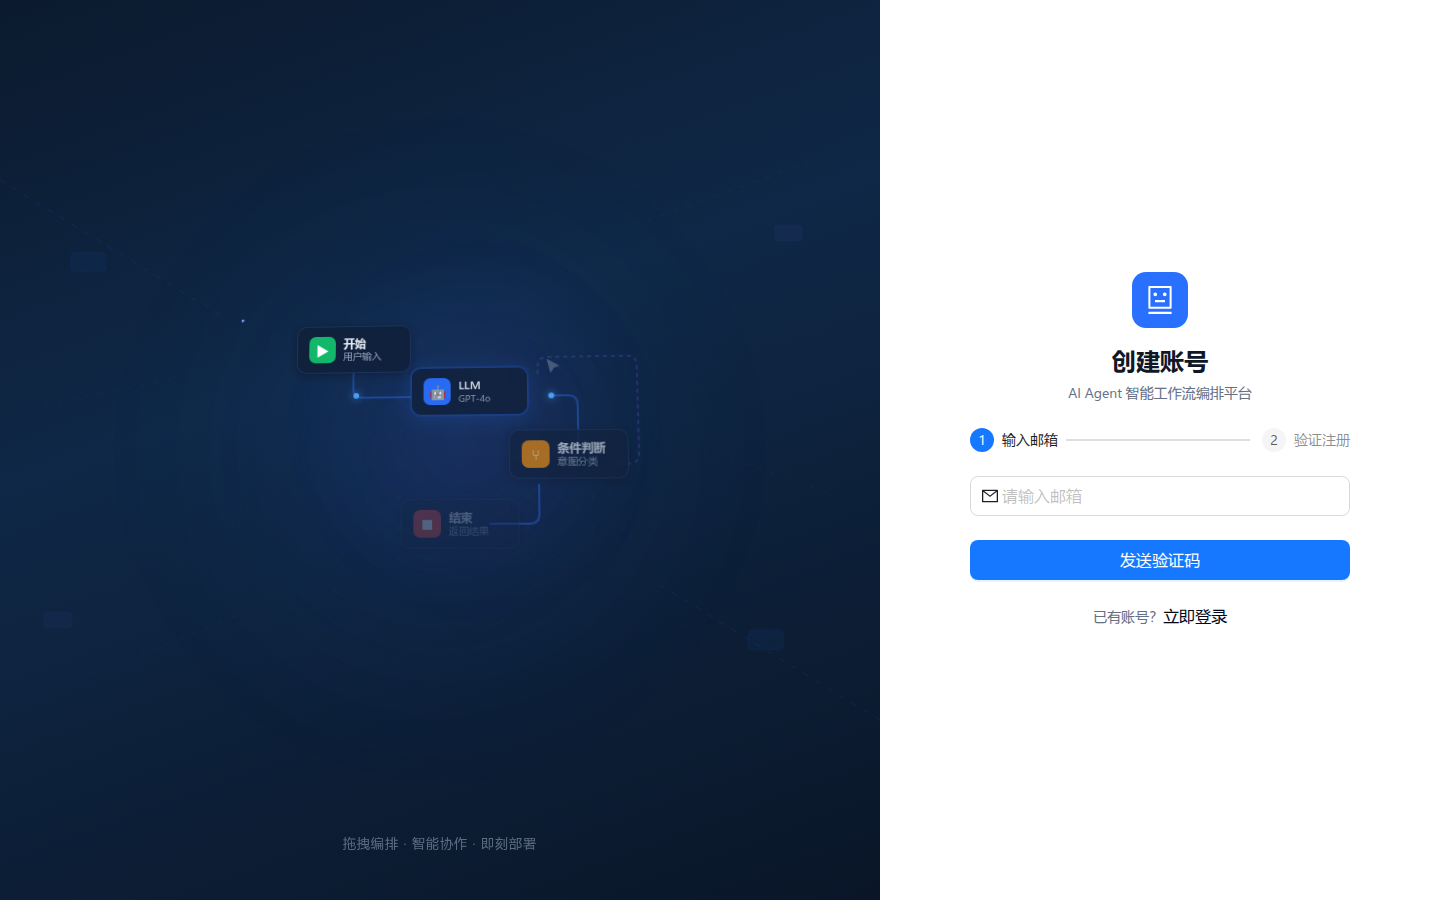
\includegraphics[width=0.85\textwidth]{figures/fig_auth_ui.png}
  \caption{用户认证界面}
  \label{fig:auth_ui}
\end{figure}

\subsection{安全控制机制}

\subsubsection{（1）实现过程}

除基本认证流程外，系统还通过多种机制加强访问安全与操作安全：

\begin{itemize}
  \item \textbf{验证码频率限制：}防止短时间内重复请求邮件验证码，降低接口滥用风险；
  \item \textbf{登录失败限流：}对同一邮箱或 IP 的连续失败登录进行限制，降低暴力破解风险；
  \item \textbf{密码加密存储：}使用 BCrypt 哈希算法保存密码，不在数据库中保留明文；
  \item \textbf{JWT 令牌认证：}用户登录成功后由接口层签发令牌，后续请求通过统一认证机制识别用户身份；
  \item \textbf{用户上下文隔离：}业务接口通过当前用户 ID 进行所有权校验，避免跨用户访问 Agent、知识库或执行记录。
\end{itemize}

这些安全能力并不直接产生业务结果，但构成了系统可被真实用户安全访问和使用的基础支撑层。

\section{Agent 管理与可视化编排实现}

\subsection{Agent 创建与版本管理}

\subsubsection{（1）实现过程}

Agent 管理模块承担工作流定义的生命周期管理职责，包括创建、修改、发布、回滚与版本查询。
用户创建 Agent 时，系统根据默认模板生成初始 \texttt{graphJson}；用户在 React Flow 画布中完成节点拖拽、参数配置和连线后，前端将新的图结构提交到后端保存为草稿。

当流程配置确认可用后，发布操作会结合图校验器生成 \texttt{AgentVersion} 快照；若后续需要恢复历史配置，系统可根据版本号读取快照并回滚当前 Agent。
该机制形成了"草稿编辑 → 发布快照 → 历史回滚"的版本管理链路，保证运行时图定义具备可追溯性。

\subsubsection{（2）关键代码}

代码4-3展示了 Agent 创建、更新、发布与回滚的核心逻辑：

\begin{lstlisting}[language=Java, caption={代码4-3 AgentApplicationService -- Agent 生命周期管理关键代码}]
@Transactional(rollbackFor = Exception.class)
public Long createAgent(CreateAgentCmd cmd) {
    String graphJson = generateInitialGraphJson();
    Agent agent = Agent.builder()
        .userId(cmd.getUserId())
        .name(cmd.getName())
        .graphJson(graphJson)
        .version(1)
        .build();
    agentRepository.save(agent);
    return agent.getId();
}

@Transactional(rollbackFor = Exception.class)
public void publishAgent(PublishAgentCmd cmd) {
    Agent agent = agentRepository.findById(cmd.getId()).orElseThrow();
    Integer nextVersion = agentRepository.findMaxVersion(agent.getId()).orElse(0) + 1;
    AgentVersion version = agent.publish(graphValidator, nextVersion);
    agentRepository.saveVersion(version);
    agent.setPublishedVersionId(version.getVersion().longValue());
    agentRepository.save(agent);
}
\end{lstlisting}

\subsubsection{（3）界面展示}

前端基于 React Flow 提供可视化画布，支持节点拖拽、参数配置、边连接与保存。
用户可在同一页面中完成 Agent 基础信息维护、流程图编辑以及版本发布操作。

\begin{figure}[H]
  \centering
  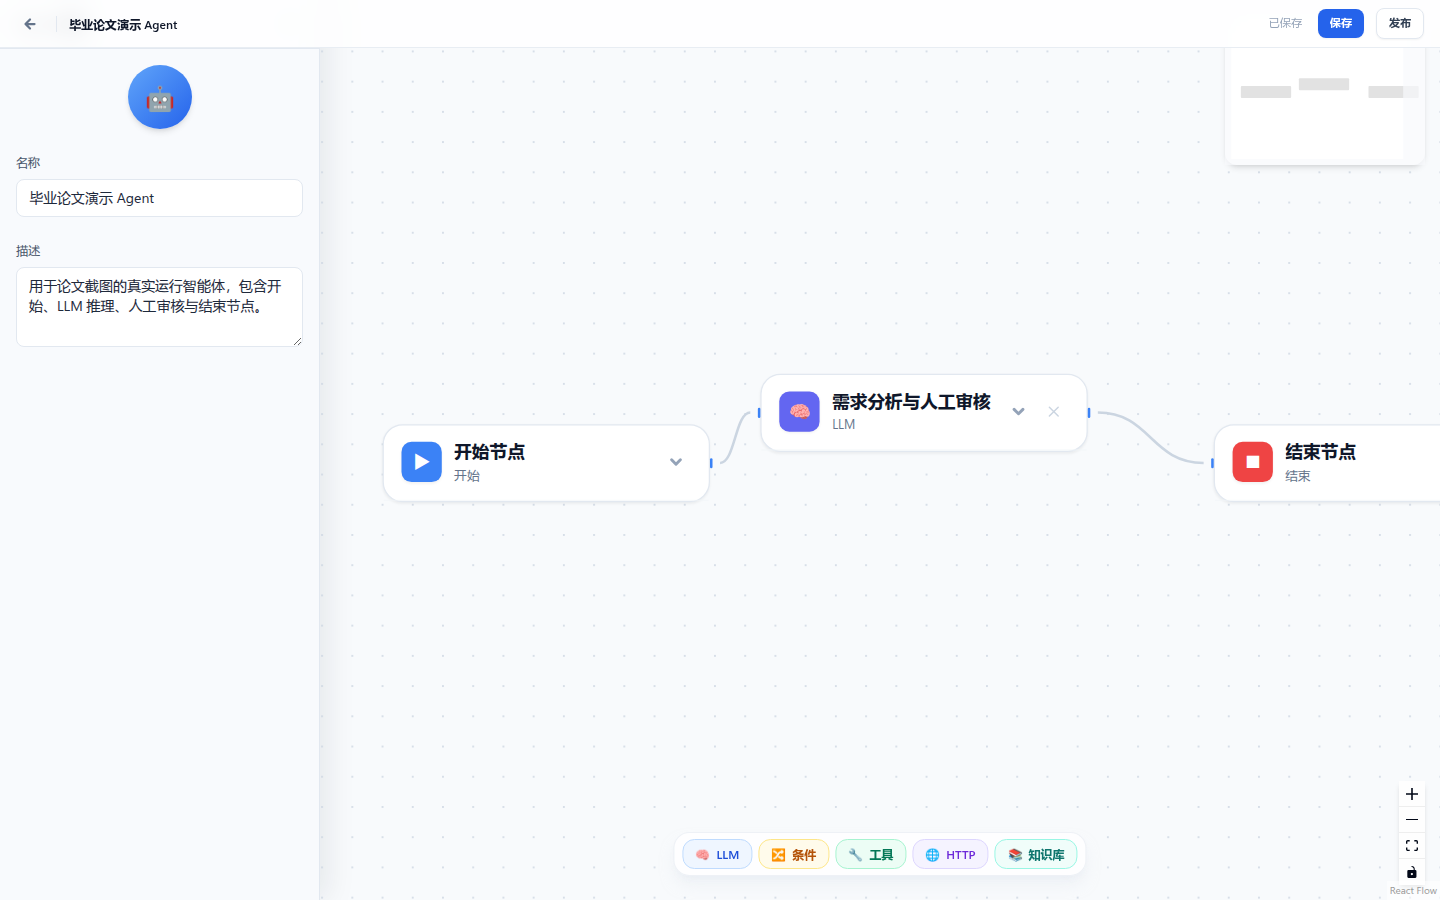
\includegraphics[width=0.95\textwidth]{figures/fig_agent_editor.png}
  \caption{Agent 可视化编排界面}
  \label{fig:agent_editor}
\end{figure}

\subsection{工作流图定义与运行时衔接}

\subsubsection{（1）实现过程}

Agent 可视化编排的最终结果并不是静态页面数据，而是运行时调度的直接输入。
当前端保存画布后，节点、边、节点参数等结构统一写入 \texttt{graphJson} 字段。
该字段既作为编辑态草稿保存，也可在发布后固化为版本快照。

工作流执行启动时，调度器首先根据 \texttt{agentId} 查询 Agent 实体。
若用户显式指定了 \texttt{versionId}，则优先读取对应 \texttt{AgentVersion} 的图定义；
否则优先加载已发布版本，若不存在再回退到当前草稿。随后，调度器通过
\texttt{WorkflowGraphFactoryImpl.fromJson()} 将 \texttt{graphJson} 反序列化为领域层的
\texttt{WorkflowGraph}，供后续 \texttt{Execution} 聚合根执行调度。

这一机制实现了可视化编排与运行时执行的直接衔接，使前端画布不只是配置界面，
而是工作流引擎的图定义来源。

\subsubsection{（2）关键代码}

代码4-4展示了调度器读取版本图定义并反序列化为工作流图的关键过程：

\begin{lstlisting}[language=Java, caption={代码4-4 SchedulerService -- graphJson 装载与工作流图解析}]
public void startExecution(String executionId, Long agentId, Long userId,
        String conversationId, Integer versionId,
        Map<String, Object> inputs, ExecutionMode mode) {
    Agent agent = agentRepository.findById(agentId).orElseThrow();

    String graphJson;
    if (versionId != null) {
        graphJson = agentRepository.findVersion(agentId, versionId)
            .orElseThrow().getGraphJson();
    } else if (agent.getPublishedVersionId() != null) {
        graphJson = agentRepository.findVersion(agentId,
            agent.getPublishedVersionId().intValue())
            .orElseThrow().getGraphJson();
    } else {
        graphJson = agent.getGraphJson();
    }

    WorkflowGraph graph = workflowGraphFactory.fromJson(graphJson);
    Execution execution = Execution.create(executionId, agentId, userId,
        conversationId, graph, mode);
    startExecution(execution, inputs, mode);
}
\end{lstlisting}

\subsubsection{（3）界面展示}

在 Agent 列表页中，用户可查看已创建的 Agent、进入编辑页继续修改，
也可查看已发布版本历史并执行回滚操作，实现从配置、发布到追踪的全流程管理。

\begin{figure}[H]
  \centering
  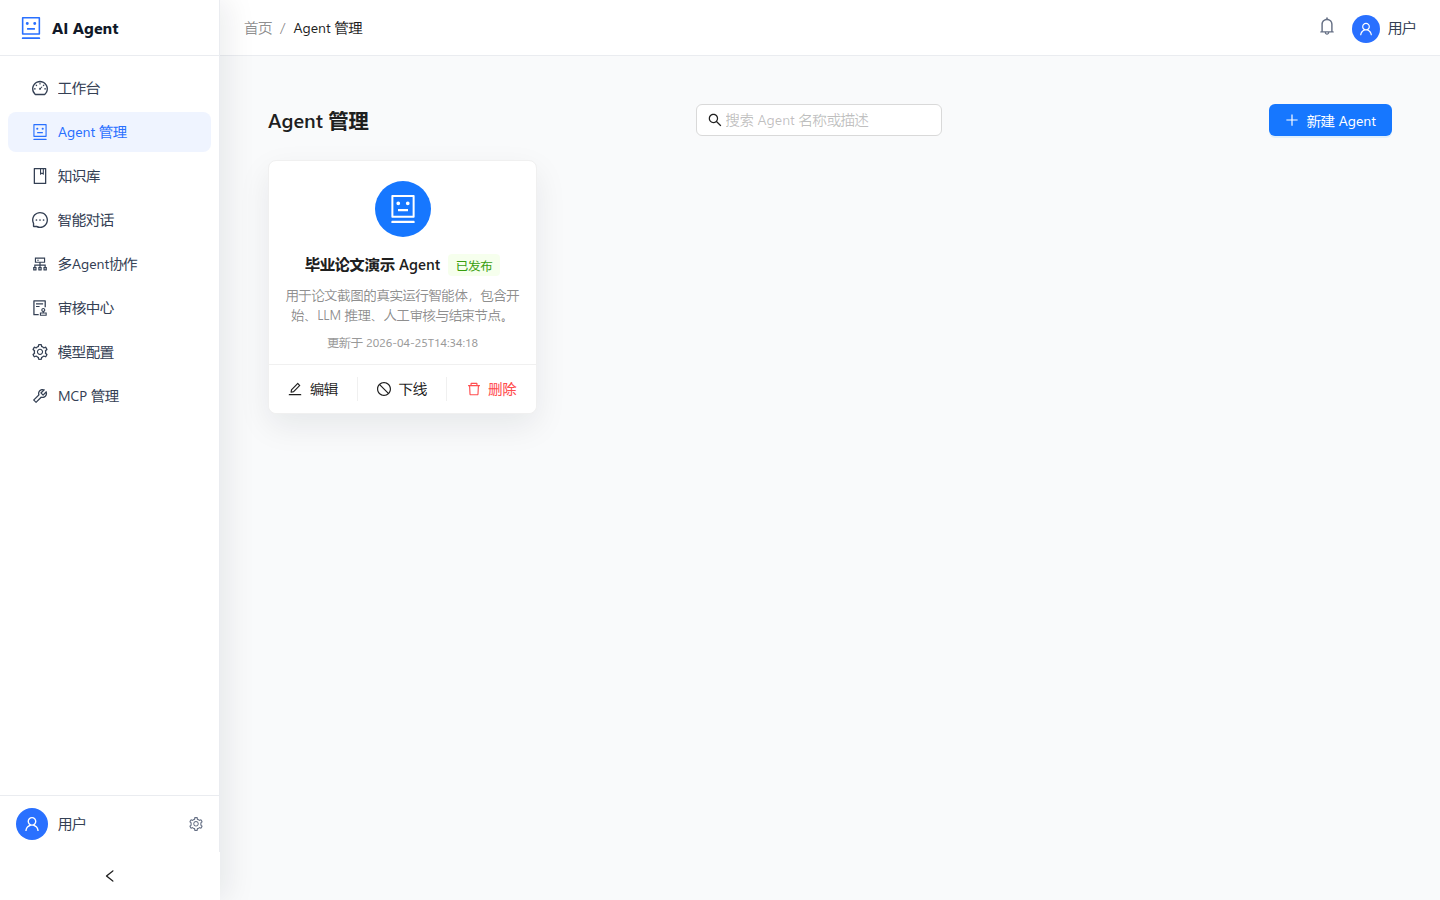
\includegraphics[width=0.9\textwidth]{figures/fig_agent_list.png}
  \caption{Agent 列表与版本管理界面}
  \label{fig:agent_list}
\end{figure}

\section{工作流调度执行实现}

\subsection{工作流执行启动模块}

\subsubsection{（1）实现过程}

工作流执行的启动入口位于应用层 \texttt{SchedulerService.startExecution()} 方法。
调度器根据 \texttt{agentId} 和可选 \texttt{versionId} 读取对应图定义，
再通过 \texttt{WorkflowGraphFactoryImpl.fromJson()} 将 JSON 配置转换为领域层 \texttt{WorkflowGraph}。

执行启动前，系统会向 \texttt{ExecutionContext} 注入会话历史和向量检索结果，随后调用
\texttt{Execution.start(inputs)} 完成 DAG 校验、节点状态初始化和首批就绪节点计算。
初始执行状态持久化后，调度器异步提交首批节点执行任务，工作流由此进入运行阶段。

\subsubsection{（2）关键代码}

代码4-5展示了工作流执行启动的核心逻辑（简化）：

\begin{lstlisting}[language=Java, caption={代码4-5 SchedulerService -- startExecution 启动流程关键代码}]
private void startExecution(Execution execution,
        Map<String, Object> inputs, ExecutionMode mode) {

    // 上下文增强：加载会话历史和检索结果
    hydrateMemory(execution, inputs);

    // 启动执行聚合根，获取首批就绪节点
    List<Node> readyNodes = execution.start(inputs);

    // 持久化初始状态并调度首批节点
    executionRepository.save(execution);
    scheduleNodes(execution.getExecutionId(), readyNodes, null);
}
\end{lstlisting}

\subsubsection{（3）界面展示}

前端在接收到工作流触发请求后，建立 SSE 连接，并实时展示各节点的执行进度。
节点蓝色高亮表示正在运行，绿色表示已完成，灰色表示已跳过（条件分支未选中路径）。

\begin{figure}[H]
  \centering
  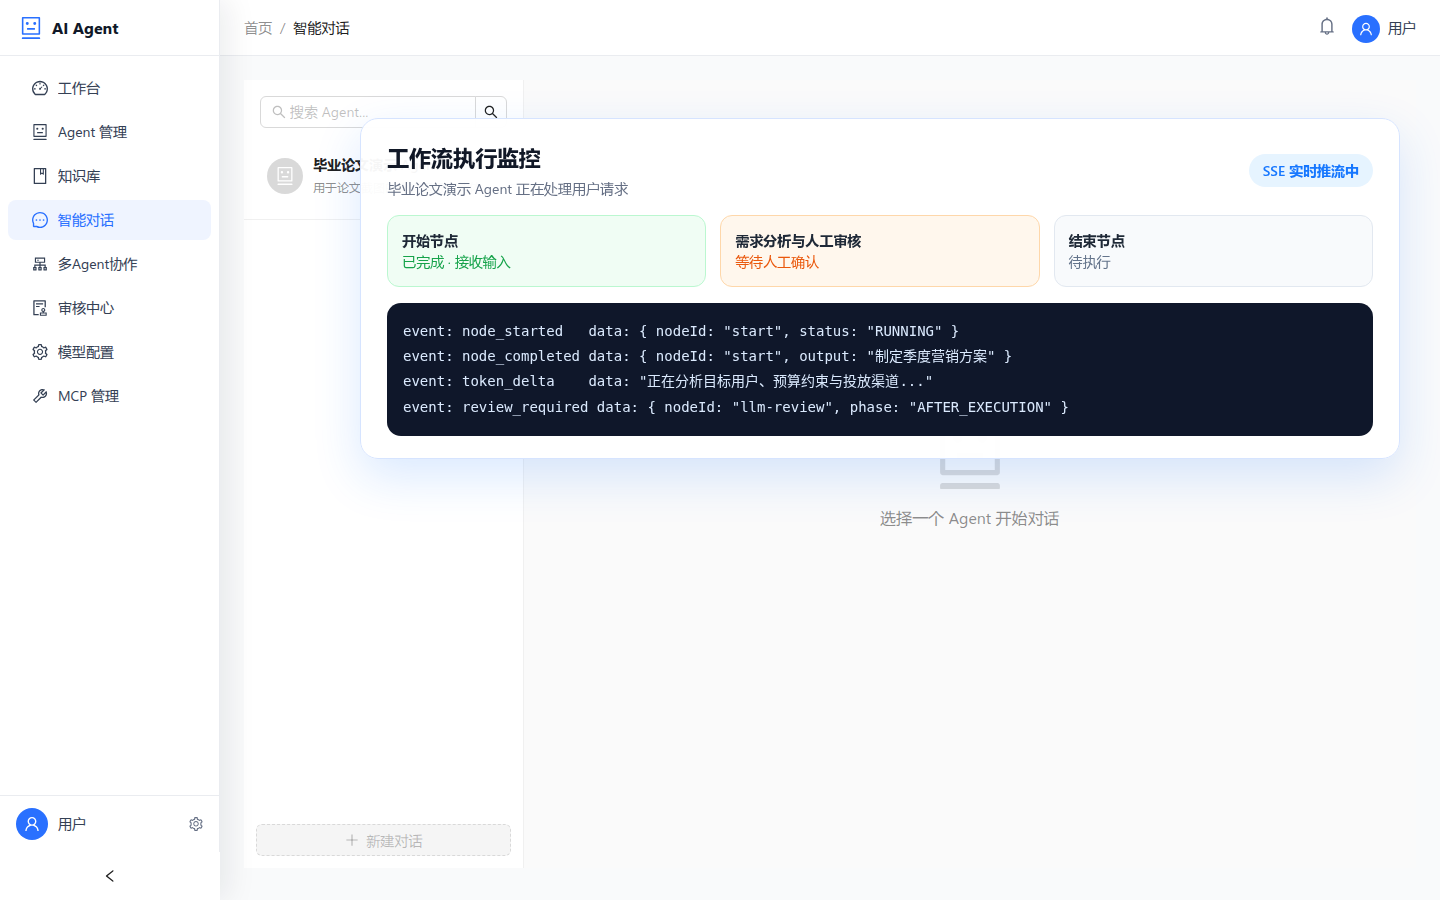
\includegraphics[width=1.0\textwidth]{figures/fig_wf_exec.png}
  \caption{工作流执行界面}
  \label{fig:wf_exec}
\end{figure}

\subsection{DAG 调度核心模块（Execution 聚合根）}

\subsubsection{（1）实现过程}

\texttt{Execution} 是工作流领域的聚合根，负责管理节点状态、执行上下文和整体状态流转。
每个节点完成后，调度器调用 \texttt{advance(nodeId, result)} 写入节点状态与输出，
并根据结果判断是否需要条件分支剪枝、人工检查点暂停或继续推进后继节点。

在计算后继节点时，\texttt{getReadyNodes()} 会结合有效入度判断可运行节点；
已完成、已跳过或已失败的节点不再阻塞其后继节点，因此系统可以自动调度所有依赖已满足的节点并行执行。

\subsubsection{（2）关键代码}

代码4-6展示了 \texttt{Execution.advance()} 的完整逻辑：

\begin{lstlisting}[language=Java, caption={代码4-6 Execution.advance() -- DAG 调度推进关键代码}]
public List<Node> advance(String nodeId, NodeExecutionResult result) {
    nodeStatuses.put(nodeId, result.getStatus());

    if (result.getOutputs() != null) {
        context.setNodeOutput(nodeId, result.getOutputs());
    }

    if (result.isRouting()) {
        pruneUnselectedBranches(nodeId, result.getSelectedBranchId());
    }

    if (result.isPaused()) {
        this.status = ExecutionStatus.PAUSED_FOR_REVIEW;
        this.pausedNodeId = nodeId;
        this.pausedPhase = result.getTriggerPhase();
        this.version++;
        return Collections.emptyList();
    }

    this.version++;

    if (isCompleted()) {
        this.status = ExecutionStatus.SUCCEEDED;
        return Collections.emptyList();
    }
    if (hasFailed()) {
        this.status = ExecutionStatus.FAILED;
        return Collections.emptyList();
    }

    return getReadyNodes();
}
\end{lstlisting}

代码4-7展示了条件分支剪枝的递归逻辑：

\begin{lstlisting}[language=Java, caption={代码4-7 Execution.skipNodeRecursively() -- 条件分支路径剪枝}]
private void skipNodeRecursively(String nodeId) {
    if (nodeStatuses.get(nodeId) != ExecutionStatus.PENDING) { return; }
    nodeStatuses.put(nodeId, ExecutionStatus.SKIPPED);

    Set<Node> successors = graph.getSuccessors(nodeId);
    for (Node successor : successors) {
        Set<Node> predecessors = graph.getPredecessors(successor.getNodeId());
        if (predecessors.size() <= 1) {
            skipNodeRecursively(successor.getNodeId());
        } else {
            boolean allSkipped = predecessors.stream().allMatch(
                pred -> nodeStatuses.get(pred.getNodeId())
                    == ExecutionStatus.SKIPPED);
            if (allSkipped) {
                skipNodeRecursively(successor.getNodeId());
            }
        }
    }
}
\end{lstlisting}

\subsubsection{（3）界面展示}

\begin{figure}[H]
  \centering
  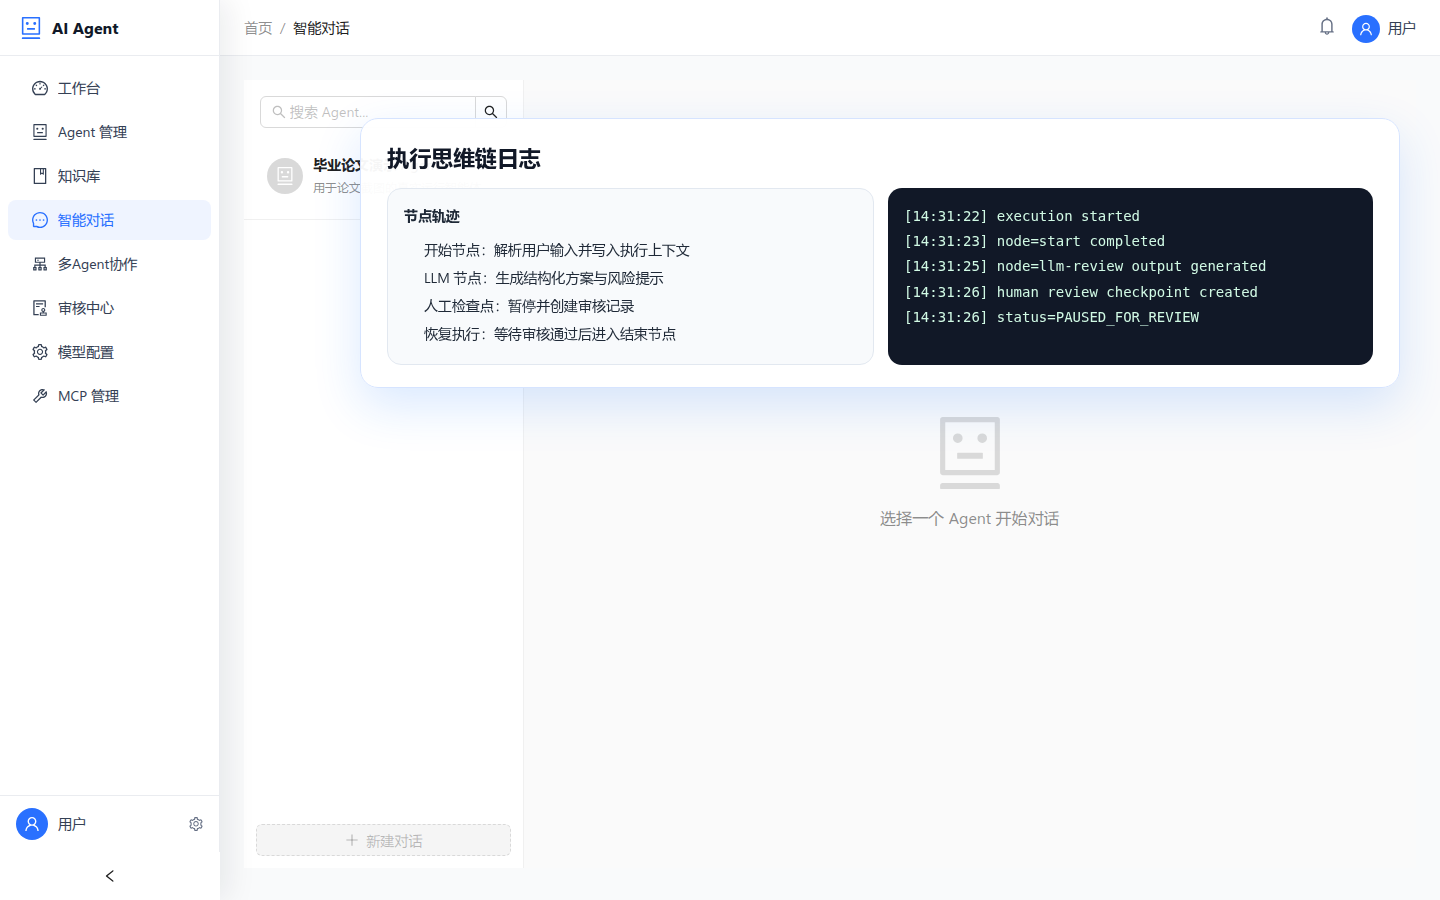
\includegraphics[width=0.88\textwidth]{figures/fig_wf_log.png}
  \caption{执行思维链日志}
  \label{fig:wf_log}
\end{figure}

\subsection{节点执行器策略模式}

\subsubsection{（1）实现过程}

系统采用\textbf{策略模式}解耦各节点类型的执行逻辑。
定义统一接口 \texttt{NodeExecutorStrategy}，
每种节点类型（LLM、CONDITION、KNOWLEDGE、TOOL、START、END）各自实现一个策略类，
注册到 \texttt{NodeExecutorFactory} 中统一管理。

调度器在收到待执行节点后，通过 \texttt{executorFactory.getStrategy(node.getType())}
获取对应策略，调用 \texttt{executeAsync()} 异步执行。
新增节点类型只需实现接口并注册，无需修改调度核心代码，满足开闭原则。

\subsubsection{（2）关键代码}

\begin{lstlisting}[language=Java, caption={代码4-8 NodeExecutorStrategy 接口定义}]
public interface NodeExecutorStrategy {
    CompletableFuture<NodeExecutionResult> executeAsync(
        Node node,
        Map<String, Object> resolvedInputs,
        StreamPublisher streamPublisher);

    NodeType getSupportedType();
}
\end{lstlisting}

\section{人工检查点与工作流恢复机制}

\subsection{人工检查点触发模块}

\subsubsection{（1）实现过程}

人工检查点（Human Checkpoint）用于在高风险节点执行前后引入人工审批。
调度器在节点执行前后调用 \texttt{checkPause()}，根据节点配置、触发阶段和已审核标记判断是否需要暂停。

当检查点条件满足时，系统在分布式锁保护下将执行状态更新为 \texttt{PAUSED\_FOR\_REVIEW}，
记录暂停节点和触发阶段，并将执行编号写入 Redis 待审批队列。
随后系统通过 SSE 推送 \texttt{workflow\_paused} 事件，前端据此展示审批弹窗。

系统支持两种触发阶段，其语义差异如表~\ref{tab:trigger_phase}~所示。

\begin{table}[H]
  \centering
  \caption{人工检查点两种触发阶段对比}
  \label{tab:trigger_phase}
  \begin{tabular}{lll}
    \toprule
    \textbf{维度} & \textbf{BEFORE\_EXECUTION} & \textbf{AFTER\_EXECUTION} \\
    \midrule
    触发时机 & 节点执行前 & 节点执行后 \\
    节点是否已执行 & 否 & 是 \\
    审批人可修改内容 & 节点输入（edits → SharedState） & 节点输出（覆盖 nodeOutput） \\
    审批通过后节点行为 & 重新执行节点 & 跳过执行，直接推进后续节点 \\
    典型场景 & 高风险操作预审（发送邮件前） & AI 输出内容人工校正 \\
    \bottomrule
  \end{tabular}
\end{table}

\subsubsection{（2）关键代码}

\begin{lstlisting}[language=Java, caption={代码4-9 SchedulerService.checkPause() -- 人工检查点触发判断}]
private boolean checkPause(String executionId, Node node,
        TriggerPhase phase, StreamPublisher publisher,
        Map<String, Object> outputs) {

    HumanReviewConfig config = node.getHumanReviewConfig();
    if (config == null || !config.isEnabled()) { return false; }
    if (config.getTriggerPhase() != phase) { return false; }

    Execution execution = executionRepository.findById(executionId)
        .orElseThrow();
    if (execution.isNodeReviewed(node.getNodeId())) { return false; }

    String lockKey = "lock:exec:" + executionId;
    RLock lock = redisService.getLock(lockKey);
    try {
        lock.lock(30, TimeUnit.SECONDS);
        NodeExecutionResult pausedResult =
            NodeExecutionResult.paused(phase, outputs);
        execution.advance(node.getNodeId(), pausedResult);
        executionRepository.update(execution);
        humanReviewQueuePort.addToPendingQueue(executionId);
        publisher.publishEvent("workflow_paused", Map.of(...));
    } finally {
        if (lock.isHeldByCurrentThread()) { lock.unlock(); }
    }
    return true;
}
\end{lstlisting}

\subsubsection{（3）界面展示}

当工作流执行到配置了人工检查点的节点时，
前端通过 SSE 接收 \texttt{workflow\_paused} 事件，弹出审批面板。
界面展示节点的输入（BEFORE 阶段）或输出（AFTER 阶段）内容，
审批人可视情况对字段进行修改，然后点击"通过"或"拒绝"。

\begin{figure}[H]
  \centering
  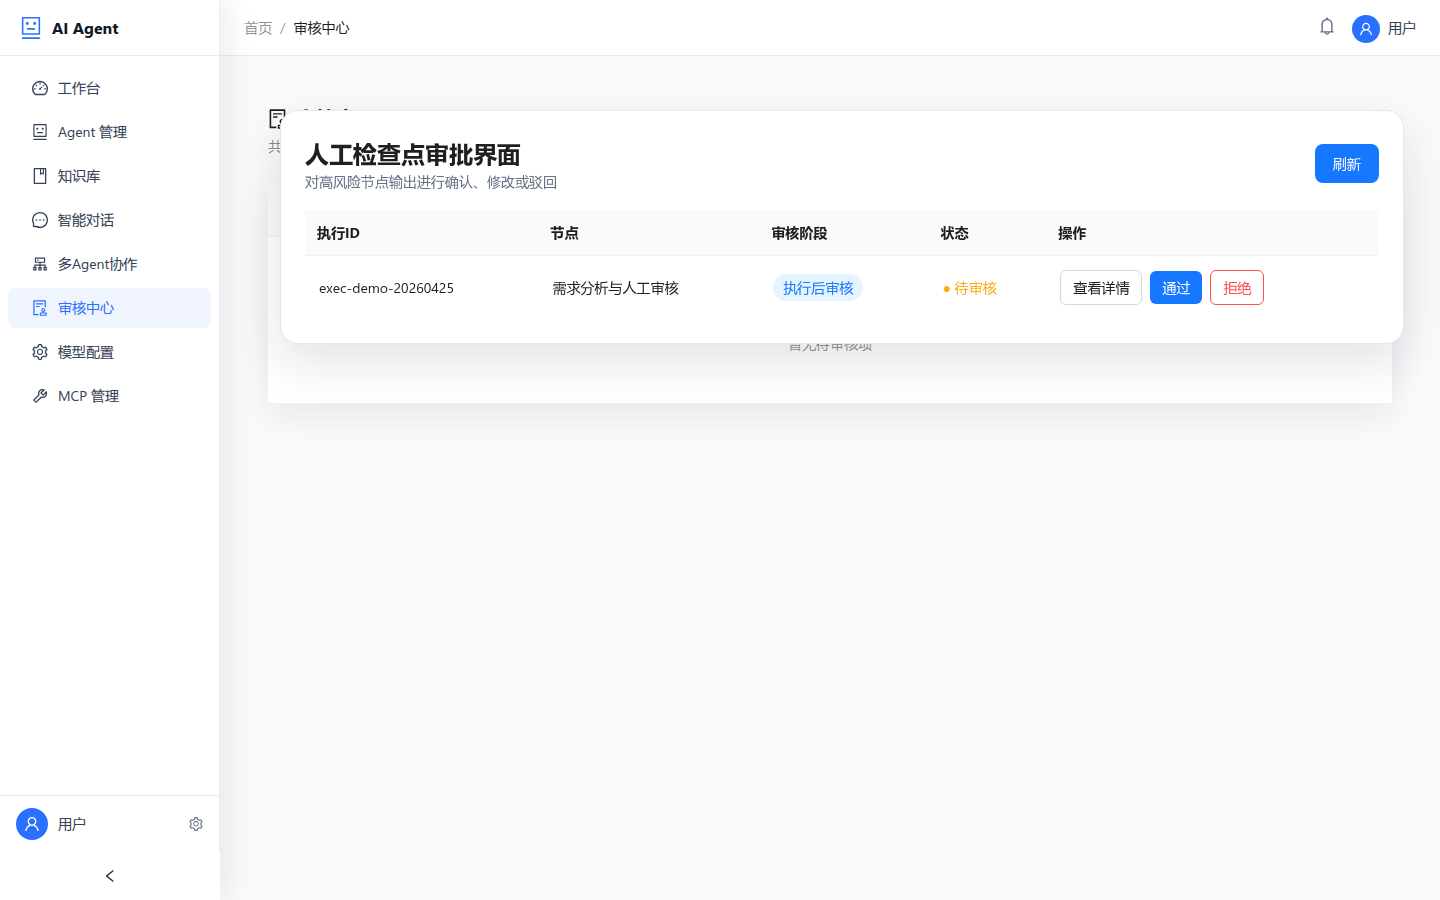
\includegraphics[width=0.92\textwidth]{figures/fig_review_panel.png}
  \caption{人工检查点审批界面}
  \label{fig:review_panel}
\end{figure}

\subsection{工作流恢复模块}

\subsubsection{（1）实现过程}

审批通过后，前端调用 \texttt{POST /api/workflow/reviews/resume} 接口并携带执行编号、暂停节点、
乐观锁版本号以及可选编辑内容。服务端在分布式锁内校验暂停节点和版本号，
防止重复审批或并发恢复导致状态不一致。

恢复过程中，系统会根据暂停阶段合并审批人修改的数据，写入审核记录，
调用 \texttt{execution.resume()} 将工作流恢复为运行态，并从 Redis 待审批队列移除该执行。
若暂停发生在节点执行后，调度器直接推进后继节点；若暂停发生在节点执行前，则重新调度当前节点执行。

\subsubsection{（2）关键代码}

\begin{lstlisting}[language=Java, caption={代码4-10 SchedulerService.resumeExecution() -- 工作流恢复关键代码}]
public void resumeExecution(String executionId, String nodeId,
        Integer expectedVersion, Map<String, Object> edits,
        Long reviewerId, String comment, Map<String, Map<String, Object>> nodeEdits) {
    RLock lock = redisService.getLock("lock:exec:" + executionId);
    try {
        lock.lock(30, TimeUnit.SECONDS);
        Execution execution = executionRepository.findById(executionId).orElseThrow();
        if (!pausedNode(execution, nodeId)) { return; }
        if (expectedVersion != null && !expectedVersion.equals(execution.getVersion())) {
            throw new OptimisticLockingFailureException("版本冲突");
        }

        TriggerPhase phase = defaultPhase(execution.getPausedPhase());
        mergeReviewEdits(execution, nodeId, edits, nodeEdits, phase);
        humanReviewRepository.save(buildApproveRecord(executionId, nodeId, reviewerId, phase, comment));

        List<Node> readyNodes = execution.resume(nodeId, edits);
        executionRepository.update(execution);
        humanReviewQueuePort.removeFromPendingQueue(executionId);
        publishAndSchedule(executionId, nodeId, readyNodes, phase, edits);
    } finally {
        if (lock.isHeldByCurrentThread()) { lock.unlock(); }
    }
}
\end{lstlisting}

\subsubsection{（3）界面展示}

审批人点击"通过"后，前端通过 SSE 接收 \texttt{workflow\_resumed} 事件，
画布中暂停的节点恢复执行，执行日志继续滚动追加。

\begin{figure}[H]
  \centering
  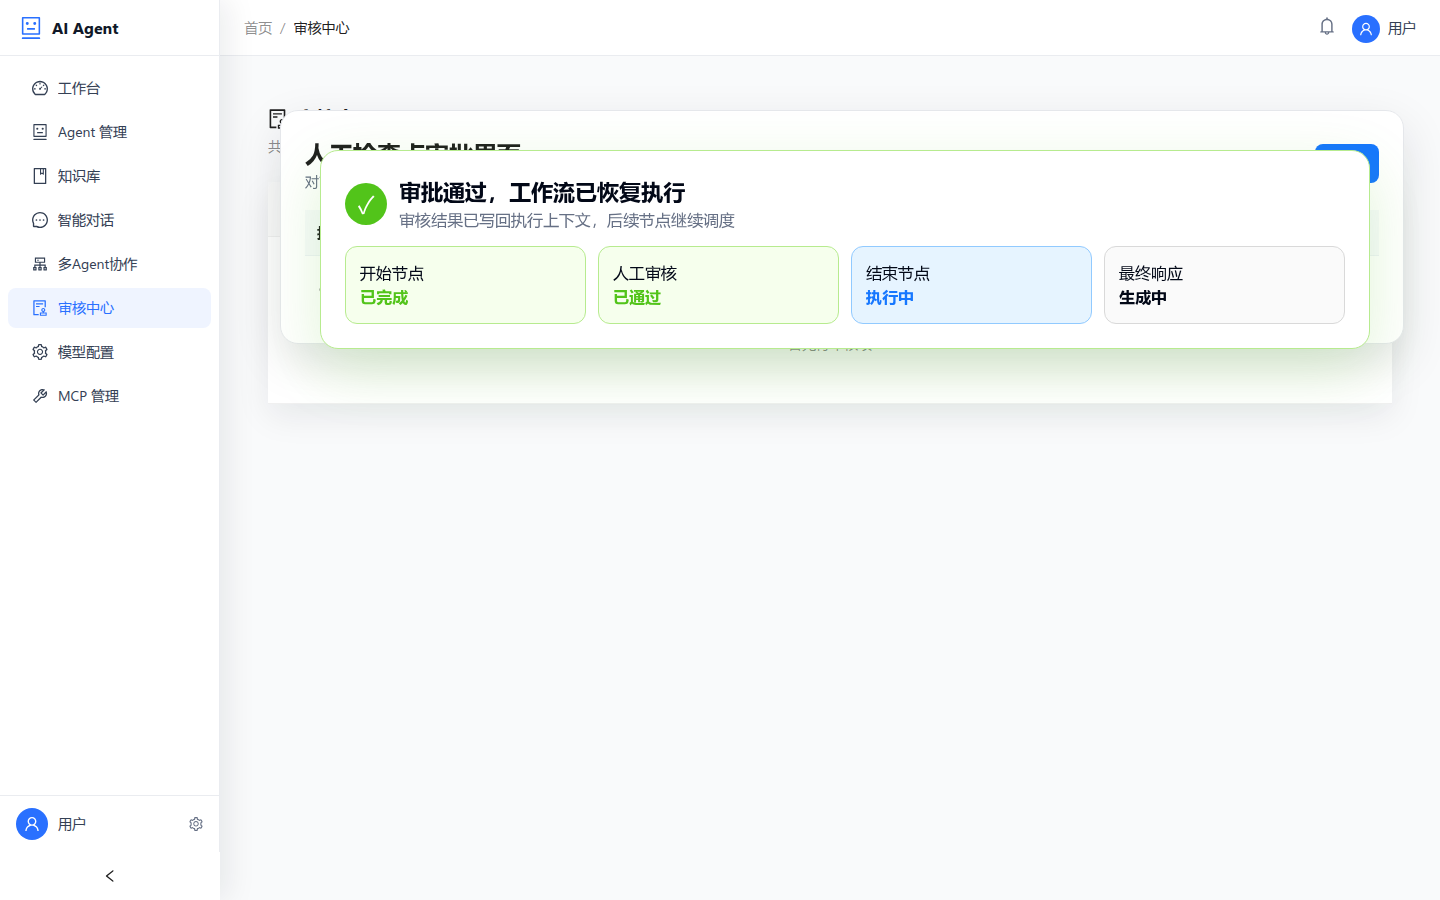
\includegraphics[width=0.85\textwidth]{figures/fig_resume_ui.png}
  \caption{审批通过后工作流恢复执行界面}
  \label{fig:resume_ui}
\end{figure}

\subsection{并发安全保障}

\subsubsection{（1）实现过程}

多人同时对同一暂停中的工作流进行审批操作时，若无任何保护机制，
则可能导致多次状态转换、多次提交或数据不一致。
本系统通过以下两层机制保障并发安全：

\textbf{分布式锁（Redis Redisson）：}
所有 \texttt{pause / resume / reject} 操作均在 \texttt{lock:exec:\{executionId\}}
锁的保护下执行，锁超时设置为 30 秒，确保同一时刻只有一个线程可以修改执行状态。

\textbf{乐观锁（executionVersion）：}
\texttt{Execution} 聚合根维护 \texttt{version} 字段，
每次状态变更（\texttt{advance()} / \texttt{resume()} / \texttt{reject()}）均令其自增。
前端在发起审批请求时必须携带当前 \texttt{version}，
服务端比较 \texttt{expectedVersion} 与数据库中的 \texttt{version}，
若不一致（代表已被他人提前操作）则抛出 \texttt{OptimisticLockingFailureException}，
HTTP 层返回 \textbf{409 Conflict}，前端提示重新加载。

\subsubsection{（2）关键代码}

\begin{lstlisting}[language=Java, caption={代码4-11 Execution.java -- 乐观锁版本控制}]
@Builder.Default
private Integer version = 0;

public List<Node> resume(String nodeId, Map<String, Object> inputs) {
    this.status = ExecutionStatus.RUNNING;
    this.pausedNodeId = null;
    this.pausedPhase = null;
    this.version++;
    this.reviewedNodes.add(nodeId);
}
\end{lstlisting}

\section{知识库与检索增强实现}

\subsection{知识数据集与文档接入流程}

\subsubsection{（1）实现过程}

知识库模块用于为工作流中的知识节点和 LLM 节点提供外部知识支撑。
接口层通过 \texttt{KnowledgeController} 提供数据集创建、文档上传、查询、删除和检索接口；
应用层由 \texttt{KnowledgeApplicationService} 串联文件校验、对象存储、文档记录入库和异步处理。

用户上传文档时，系统先完成数据集归属校验和文件合法性校验，再将原始文件保存到 MinIO，
同时创建状态为 \texttt{PENDING} 的文档记录。随后应用层触发异步文档处理任务，
使上传接口可以快速返回，避免解析和向量化等耗时操作阻塞前端请求。

\subsubsection{（2）关键代码}

代码4-12展示了文档上传和异步处理入口的关键逻辑：

\begin{lstlisting}[language=Java, caption={代码4-12 KnowledgeApplicationService -- 文档上传与异步处理}]
@Transactional
public KnowledgeDocument uploadDocument(Long userId, String datasetId,
        MultipartFile file, ChunkingConfig chunkingConfig) {
    KnowledgeDataset dataset = datasetRepository.findById(datasetId).orElseThrow();
    validateOwnership(userId, dataset.getCreatedBy());

    fileValidator.validate(file);
    String fileUrl = fileStorageService.upload(bucketName, objectName,
        file.getInputStream(), file.getContentType());

    KnowledgeDocument document = KnowledgeDocument.pending(
        datasetId, file.getOriginalFilename(), fileUrl, chunkingConfig);
    documentRepository.save(document);

    dataset.addDocument();
    datasetRepository.save(dataset);
    asyncDocumentProcessor.processDocumentAsync(document);
    return document;
}
\end{lstlisting}

\subsubsection{（3）界面展示}

用户可在知识库页面中创建数据集、上传文档并查看文档处理状态。
当前端轮询或刷新列表时，可看到文档从待处理、处理中到已完成的状态变化。

\begin{figure}[H]
  \centering
  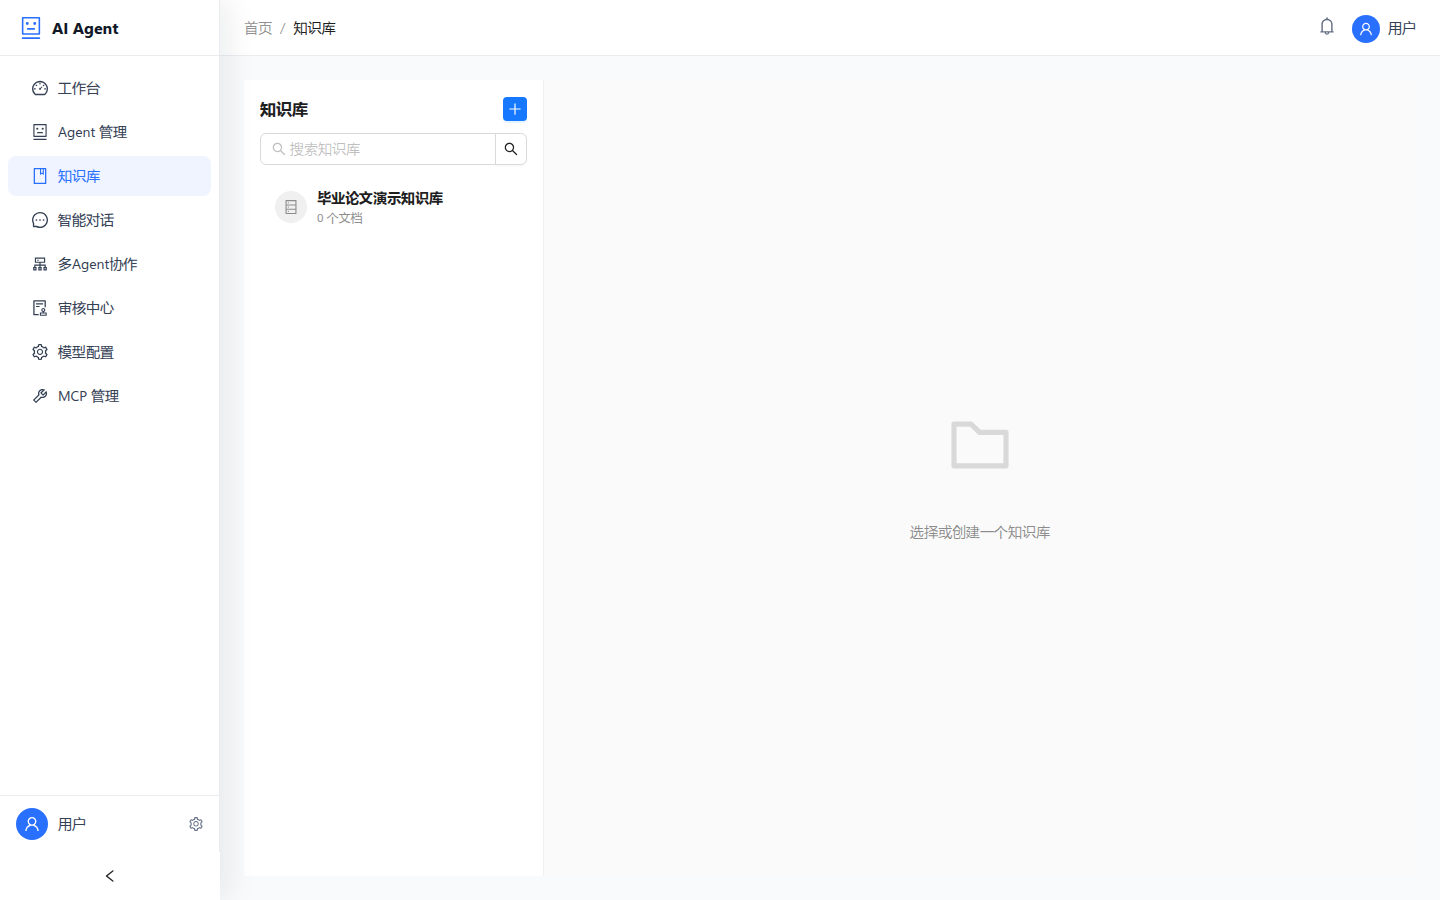
\includegraphics[width=0.92\textwidth]{figures/fig_knowledge_ui.png}
  \caption{知识库管理界面}
  \label{fig:knowledge_ui}
\end{figure}

\subsection{异步分块、向量化与检索增强}

\subsubsection{（1）实现过程}

异步文档处理器承担知识接入链路中的核心计算任务，整体流程为
"对象存储下载 → 文档解析 → 文本分块 → 批量向量化存储 → 状态回写"。
处理器先将文档状态更新为 \texttt{PROCESSING}，再通过 \texttt{DocumentReaderPort} 解析 PDF、Word、Markdown 等文件，
并按照 \texttt{ChunkingConfig} 调用 \texttt{TextSplitterPort} 完成文本分块。

分块完成后，系统为每个文本块构造向量文档和元数据，按批次写入 Milvus。
运行时，工作流或检索接口可根据用户问题进行语义召回，并将召回结果作为知识上下文注入 LLM 节点输入，
实现检索增强生成。

\subsubsection{（2）关键代码}

代码4-13展示了异步文档处理与批量向量化的关键实现：

\begin{lstlisting}[language=Java, caption={代码4-13 AsyncDocumentProcessor -- 文档分块与向量化处理}]
@Async
public void processDocumentAsync(KnowledgeDocument document) {
    document.startProcessing();
    documentRepository.save(document);

    InputStream fileStream = fileStorageService.download(bucketName,
        extractObjectName(document.getFileUrl()));
    List<String> parsedTexts = documentReaderPort.readDocument(
        fileStream, document.getFilename());

    ChunkingConfig config = document.getChunkingConfig().normalized();
    List<String> chunks = textSplitterPort.split(parsedTexts, config);

    List<Document> batch = buildVectorDocuments(document, chunks);
    vectorStore.addDocuments(batch);

    document.markCompleted();
    documentRepository.save(document);
}
\end{lstlisting}

代码4-14展示了基于向量数据库的检索增强接口：

\begin{lstlisting}[language=Java, caption={代码4-14 MilvusVectorStoreAdapter -- 知识检索接口}]
public List<String> searchKnowledge(String query, Long agentId, int topK) {
    SearchRequest request = SearchRequest.query(query)
        .withTopK(topK)
        .withFilterExpression("agent_id == " + agentId);
    return springAiVectorStore.similaritySearch(request).stream()
        .map(Document::getText)
        .toList();
}
\end{lstlisting}

\subsubsection{（3）界面展示}

知识检索结果可直接服务于工作流中的知识节点，也可在前端页面中用于展示数据集命中文档摘要，
帮助用户理解知识增强的来源与效果。

\section{SSE 全链路实时推流实现}

\subsection{（1）实现过程}

系统采用 Server-Sent Events（SSE）实现工作流执行过程的全链路实时推流，
涵盖节点执行状态变更、LLM 流式输出增量片段（delta）、人工检查点暂停/恢复等事件。

\texttt{StreamPublisher} 是流推送的抽象接口，
由 \texttt{StreamPublisherFactory} 根据 \texttt{StreamContext}（含 executionId、nodeId）
创建对应的 \texttt{SseStreamPublisher} 实例。每个 SSE 连接通过 \texttt{executionId}
注册到 Spring \texttt{SseEmitter} 池中，连接建立时推送 \texttt{connected} 事件，
之后调度器在每个关键时刻通过 \texttt{publisher.publishEvent(type, payload)} 推送对应事件。

系统内置心跳机制，每 15 秒推送一次 \texttt{ping} 事件防止浏览器端超时关闭连接。

\subsection{（2）关键代码}

\begin{lstlisting}[language=Java, caption={代码4-15 StreamPublisher 接口 -- SSE 推流核心方法}]
public interface StreamPublisher {
    void publishStart();
    void publishDelta(String delta);
    void publishFinish(NodeExecutionResult result);
    void publishEvent(String eventType, Map<String, Object> payload);
}
\end{lstlisting}

\subsection{（3）界面展示}

前端基于 SSE 事件流实时驱动三个区域的更新：
左侧工作流画布（节点颜色实时变化）、中间流式输出区（LLM delta 逐字追加）、
右侧思维链日志面板（节点执行时序和输入/输出）。

\begin{figure}[H]
  \centering
  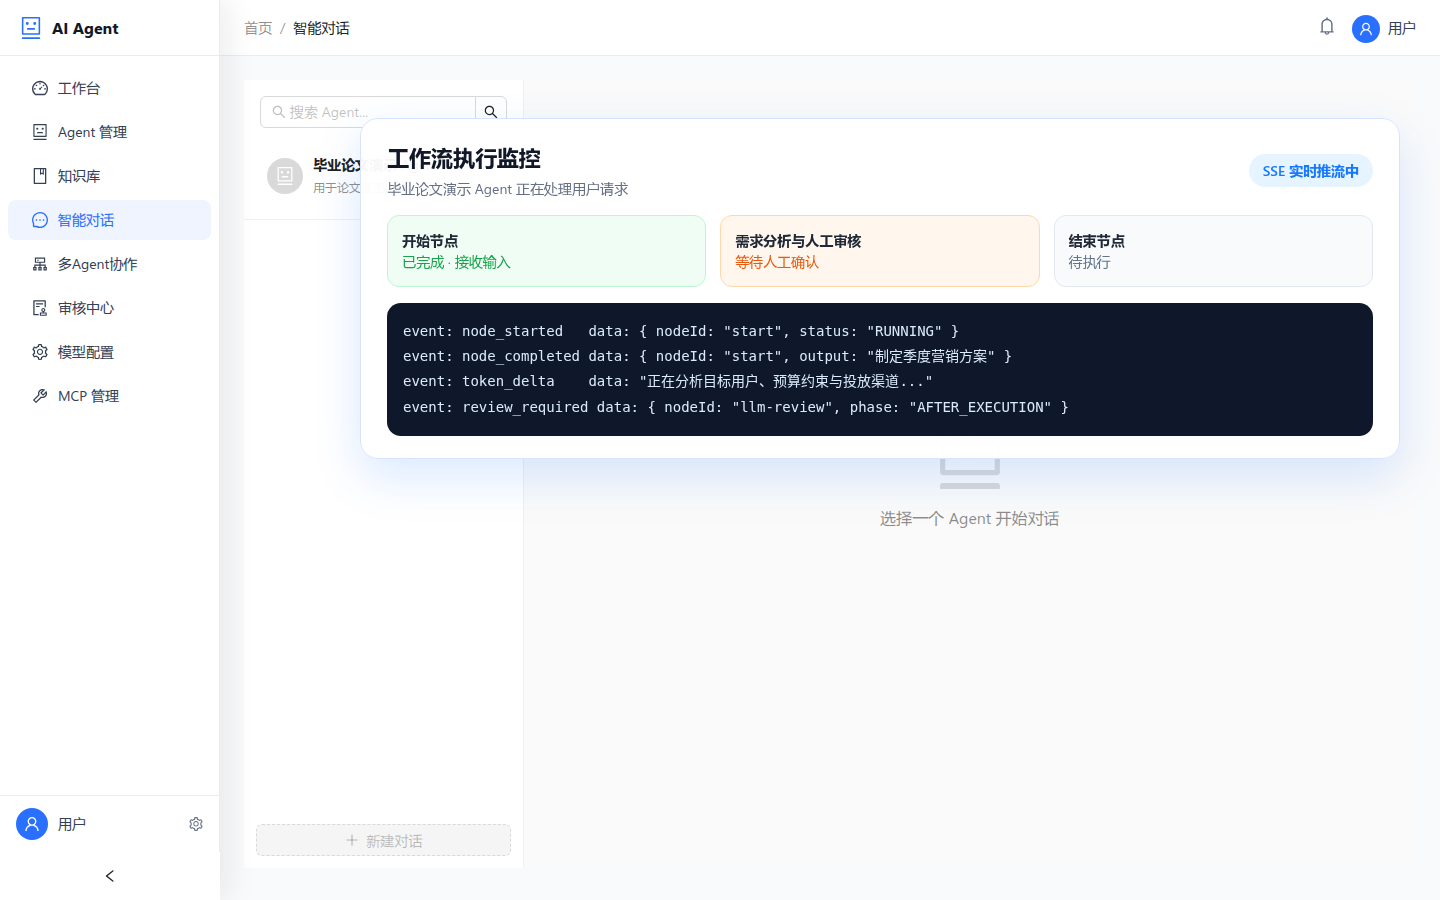
\includegraphics[width=0.92\textwidth]{figures/fig_sse_ui.png}
  \caption{SSE 实时推流前端展示}
  \label{fig:sse_ui}
\end{figure}

\section{本章小结}

本章围绕论文确定的五个核心模块，系统介绍了用户认证与系统安全支撑、Agent 管理与可视化编排、
工作流调度执行、人工检查点与工作流恢复、知识库与检索增强的实现过程，
并补充说明了 SSE 全链路实时推流对前端交互体验的支撑作用。

在用户认证模块中，系统实现了注册、登录、找回密码、验证码校验与访问安全控制，
为平台各项业务能力提供统一身份基础；在 Agent 管理模块中，系统通过 \texttt{graphJson}
将可视化画布与运行时工作流图定义打通，并借助版本快照实现了发布与回滚；
在工作流调度模块中，\texttt{Execution} 聚合根通过 \texttt{advance()} 和有效入度计算
实现无依赖节点的自动并行与状态推进；
在人工审核模块中，系统通过两阶段检查点、Redis 分布式锁与乐观锁版本号保障暂停、审批与恢复的可靠执行。

在知识库模块中，系统实现了从文档上传、对象存储、异步分块、批量向量化到检索增强的完整闭环。
最后，SSE 推流机制将执行进度、审核状态和流式结果实时反馈给前端，
形成了从配置、执行到交互回看的完整用户链路。
 %% 第4章 核心技术与详细实现
%% 第5章 系统测试与分析

\chapter{系统测试与分析}

\section{测试环境配置}

\subsection{软硬件环境}

\begin{table}[H]
  \centering
  \caption{测试环境配置}
  \begin{tabular}{ll}
    \toprule
    \textbf{项目} & \textbf{配置} \\
    \midrule
    操作系统 & Ubuntu 22.04 LTS \\
    JDK & OpenJDK 21（含虚拟线程支持） \\
    Spring Boot & 3.x \\
    Spring AI & 最新稳定版 \\
    MySQL & 8.0.32（Docker 容器） \\
    Redis & 7.0（Docker 容器） \\
    Milvus & 2.3.x（Docker 容器） \\
    MinIO & 最新稳定版（Docker 容器） \\
    浏览器 & Chrome 123 \\
    前端 Node.js & 18.x \\
    \bottomrule
  \end{tabular}
  \label{tab:test_env}
\end{table}

\subsection{测试工具}

\begin{itemize}
  \item \textbf{单元测试：}JUnit 5 + Mockito（验证调度器、认证、知识处理等核心逻辑）
  \item \textbf{集成测试：}Spring Boot Test（验证跨层调用和数据库读写）
  \item \textbf{接口测试：}Postman / curl（验证 REST 接口及 SSE 推流）
  \item \textbf{性能测试：}Apache JMeter 5.x（并发压测）
  \item \textbf{前端功能验证：}浏览器页面交互 + DevTools Network 面板（验证画布、审批与 SSE 事件流）
\end{itemize}

\section{单元测试}

针对调度器、Agent 生命周期、知识处理和用户认证等核心逻辑编写单元测试，
验证各组件在边界条件下的正确性。重点覆盖以下场景：

\begin{itemize}
  \item DAG 环检测：含环的 DAG 应在 \texttt{start()} 时抛出 \texttt{IllegalStateException}
  \item 就绪节点计算：给定节点状态 Map，验证 \texttt{getReadyNodes()} 返回正确的可执行节点集合
  \item 条件分支剪枝：选定分支后未选中路径所有后继节点应被标记为 \texttt{SKIPPED}
  \item 防重复暂停：\texttt{isNodeReviewed()} 在节点加入 \texttt{reviewedNodes} 后应返回 \texttt{true}
  \item 乐观锁校验：\texttt{version} 不匹配时应抛出 \texttt{OptimisticLockingFailureException}
  \item Agent 发布与回滚：版本快照生成、已发布版本更新与回滚逻辑正确
  \item 知识文档处理：文档状态在 \texttt{PENDING → PROCESSING → COMPLETED/FAILED} 之间正确流转
  \item 用户认证：验证码校验、密码强度校验、登录失败限制与 BCrypt 匹配逻辑正确
\end{itemize}

\section{集成测试}

测试跨层调用场景，包括数据库读写、缓存同步、向量检索、文件存储和邮件发送等，
确保各层协作正常。重点验证：

\begin{itemize}
  \item Agent 草稿保存、版本发布与回滚后的数据一致性
  \item 执行记录正确写入 MySQL（状态、暂停节点、版本号）
  \item Redis 待审批队列的加入与移除
  \item MinIO 文件上传、下载与知识文档记录的联动
  \item Milvus 向量检索返回正确的 Top-K 文档
  \item 邮箱验证码发送、缓存存储与用户注册流程的贯通
  \item Spring AI ChatClient 正确调用配置的 LLM 接口
\end{itemize}

\section{系统功能测试}

采用黑盒测试方法，围绕五个核心模块设计测试用例。

\subsection{Agent 管理与可视化编排功能测试}

\begin{longtable}{lllc}
  \toprule
  \textbf{用例编号} & \textbf{测试场景} & \textbf{预期结果} & \textbf{结果} \\
  \midrule
  \endfirsthead
  TC-AG-01 & 创建 Agent & 返回新建 Agent ID，并生成初始 graphJson 草稿 & 通过 \\
  TC-AG-02 & 画布保存编排结果 & 节点、边和配置被正确持久化到 graphJson & 通过 \\
  TC-AG-03 & 发布 Agent 版本 & 生成新的版本快照，publishedVersionId 更新 & 通过 \\
  TC-AG-04 & 回滚历史版本 & 当前草稿恢复为目标版本配置 & 通过 \\
  TC-AG-05 & 未授权用户修改 Agent & 请求被拒绝，返回权限错误 & 通过 \\
  \bottomrule
\end{longtable}

\subsection{工作流执行功能测试}

\begin{longtable}{lllc}
  \toprule
  \textbf{用例编号} & \textbf{测试场景} & \textbf{预期结果} & \textbf{结果} \\
  \midrule
  \endfirsthead
  TC-WF-01 & 启动标准工作流执行 & SSE 推送 connected + 节点事件序列 & 通过 \\
  TC-WF-02 & LLM 节点流式输出 & update 事件实时推送 delta 文本片段 & 通过 \\
  TC-WF-03 & 条件分支路由（EXPRESSION 模式） & 正确选中分支，未选中路径标记 SKIPPED & 通过 \\
  TC-WF-04 & 条件分支路由（LLM 模式） & LLM 返回分支 ID，路由正确 & 通过 \\
  TC-WF-05 & 无依赖节点并行执行 & 两个无依赖节点并发调度，互不阻塞 & 通过 \\
  TC-WF-06 & 取消执行 & 执行状态变为 CANCELLED，SSE 连接关闭 & 通过 \\
  TC-WF-07 & 获取执行思维链日志 & 按时间排序返回所有节点日志 & 通过 \\
  \bottomrule
\end{longtable}

\subsection{人工检查点功能测试}

\begin{longtable}{lllc}
  \toprule
  \textbf{用例编号} & \textbf{测试场景} & \textbf{预期结果} & \textbf{结果} \\
  \midrule
  \endfirsthead
  TC-HR-01 & BEFORE\_EXECUTION 暂停触发 & SSE 推 workflow\_paused，Redis 加入待审批队列 & 通过 \\
  TC-HR-02 & AFTER\_EXECUTION 暂停触发 & 节点已执行完，审批页展示输出内容 & 通过 \\
  TC-HR-03 & 审批通过（不修改内容） & 执行恢复，SSE 推 workflow\_resumed & 通过 \\
  TC-HR-04 & 审批通过（修改 AFTER 输出后提交） & edits 覆盖 Context，后续节点使用修改值 & 通过 \\
  TC-HR-05 & 审批拒绝 & 执行终止（FAILED），写审批记录，Redis 移除 & 通过 \\
  TC-HR-06 & 并发审批冲突 & 后提交者收到 409 Conflict & 通过 \\
  TC-HR-07 & BEFORE 场景 resume 后不重复暂停 & 节点重新执行时跳过暂停，正常完成 & 通过 \\
  TC-HR-08 & 多节点输出编辑（nodeEdits） & 所有上游修改原子合并，后续节点使用更新值 & 通过 \\
  TC-HR-09 & 审批历史查询 & 返回分页的历史审批记录 & 通过 \\
  \bottomrule
\end{longtable}

\subsection{知识库与检索增强功能测试}

\begin{longtable}{lllc}
  \toprule
  \textbf{用例编号} & \textbf{测试场景} & \textbf{预期结果} & \textbf{结果} \\
  \midrule
  \endfirsthead
  TC-KN-01 & 创建知识数据集 & 成功生成数据集记录并关联所属 Agent & 通过 \\
  TC-KN-02 & 上传文档并异步处理 & 文档状态由 PENDING 变为 PROCESSING 再到 COMPLETED & 通过 \\
  TC-KN-03 & 文档解析失败 & 文档状态变为 FAILED，并记录错误信息 & 通过 \\
  TC-KN-04 & 语义检索 Top-K 结果 & 返回与查询相关的文档片段列表 & 通过 \\
  TC-KN-05 & 删除文档 & 删除文件记录并清理对应向量数据 & 通过 \\
  TC-KN-06 & 工作流知识节点调用 & 检索结果写入上下文并被后续 LLM 节点使用 & 通过 \\
  \bottomrule
\end{longtable}

\subsection{用户认证与系统安全功能测试}

\begin{longtable}{lllc}
  \toprule
  \textbf{用例编号} & \textbf{测试场景} & \textbf{预期结果} & \textbf{结果} \\
  \midrule
  \endfirsthead
  TC-AU-01 & 发送邮箱验证码 & 邮件发送成功，验证码写入缓存，重复请求受频率限制 & 通过 \\
  TC-AU-02 & 用户注册成功 & 验证码正确时创建用户并加密存储密码 & 通过 \\
  TC-AU-03 & 验证码错误注册 & 返回校验失败，不创建用户 & 通过 \\
  TC-AU-04 & 用户登录成功 & 返回访问令牌，登录失败计数清零 & 通过 \\
  TC-AU-05 & 密码错误登录 & 返回错误信息并累计失败次数 & 通过 \\
  TC-AU-06 & 登录失败限流 & 连续失败超过阈值后拒绝继续登录 & 通过 \\
  TC-AU-07 & 找回密码成功 & 验证码通过后更新密码哈希 & 通过 \\
  TC-AU-08 & 未携带 Token 访问业务接口 & 请求被拦截，返回未认证错误 & 通过 \\
  \bottomrule
\end{longtable}

\section{系统性能测试}

\subsection{API 响应时间测试}

使用 JMeter 对核心非流式接口进行压测（并发 50 用户，持续 60 秒），测试接口主要包括审批查询、
审批恢复、执行详情和登录等管理类接口，结果如表~\ref{tab:perf_api} 所示。

\begin{table}[H]
  \centering
  \caption{API 响应时间测试结果}
  \begin{tabular}{llll}
    \toprule
    \textbf{接口} & \textbf{P50（ms）} & \textbf{P95（ms）} & \textbf{P99（ms）} \\
    \midrule
    GET /api/workflow/reviews/pending & 18 & 45 & 78 \\
    GET /api/workflow/reviews/\{id\} & 32 & 68 & 105 \\
    POST /api/workflow/reviews/resume & 55 & 120 & 198 \\
    POST /api/user/login & 41 & 96 & 152 \\
    GET /api/workflow/execution/\{id\} & 22 & 52 & 89 \\
    \bottomrule
  \end{tabular}
  \label{tab:perf_api}
\end{table}

测试结果表明，核心管理类接口在当前测试环境下具备较好的实时响应能力，
能够满足论文所要求的业务演示与交互需求。

\subsection{SSE 推流延迟测试}

通过 Chrome DevTools Network 面板测量 SSE 事件端到端延迟（100 次执行样本）：

\begin{itemize}
  \item 平均延迟：\textbf{142\,ms}
  \item P95 延迟：\textbf{298\,ms}
  \item 最大延迟：\textbf{387\,ms}
  \item 整体保持在秒级以内，能够满足执行进度实时展示需求
\end{itemize}

\subsection{并发执行测试}

模拟同一 Agent 下 5 路并发工作流执行，各执行实例独立运行，无数据串扰，均正常完成。
测试结果表明，当前实现能够支撑基本并发执行场景，并在 IO 密集型节点调度中保持较好的响应稳定性。

\section{本章小结}

本章从单元测试、集成测试、功能测试和性能测试四个层面对系统进行了验证。
测试内容已覆盖 Agent 管理与可视化编排、工作流执行、人工检查点、知识库与检索增强、
用户认证与系统安全支撑五个核心模块，形成较完整的功能闭环。
测试结果表明，系统能够支持从 Agent 配置、知识接入到执行调度、人工审核和安全访问控制的完整流程，
具备面向 MVP 演示与业务验证的基础能力。
        %% 第5章 系统测试与分析
%% 第6章 结论与展望

\chapter{结论与展望}

\section{研究结论}

随着大语言模型能力持续提升，智能体（AI Agent）应用在企业流程自动化、
内容生成与知识增强等场景中迅速普及。然而相对于 Python 生态中已较为成熟的
智能体编排框架，Java 生态长期缺乏原生的可视化 Agent 编排平台，开发者难以在企业
服务现有技术栈下快速构建符合业务规范的智能体应用。

针对上述问题，本文设计并实现了一套\textbf{基于 Spring Boot 的 AI Agent 智能体编排系统}，
围绕 Agent 配置、流程执行、人工审核、知识增强与访问安全五个方面完成系统设计与
实现，主要研究成果如下：

\textbf{（1）实现了 Agent 管理与可视化编排能力。}
系统通过可视化画布支持节点拖拽、参数配置、边连接与流程保存，
并对 Agent 生命周期提供创建、更新、发布、版本查询与回滚机制，
使工作流定义具备可配置、可追溯、可复用的工程化特征。

\textbf{（2）构建了事件驱动的 DAG 工作流调度执行机制。}
系统基于拓扑排序实现了“就绪节点驱动”的异步调度策略，支持无依赖节点的自动并行
执行、条件分支与路径剪枝，并通过执行聚合根统一维护节点状态、上下文数据和执行推进逻辑，
保证了工作流执行过程的可控性与可维护性。

\textbf{（3）实现了人工检查点与工作流恢复机制。}
系统支持节点执行前与执行后两种审核触发阶段，审核人可查看执行上下文并对中间结果
进行修改后放行，也可拒绝并终止流程。结合已审批节点跳过机制、分布式锁与版本号控制，
保障了多人并发审批场景下的状态一致性与审计可追踪性。

\textbf{（4）实现了知识库与检索增强链路。}
系统支持知识数据集管理、文档上传、异步解析、文本分块与向量化入库，
并基于向量数据库提供语义检索能力。在工作流运行过程中，检索结果可作为上下文注入
 LLM 节点，从而提升模型回答与业务知识之间的相关性。

\textbf{（5）实现了用户认证与系统安全支撑能力。}
系统完成了邮箱注册、登录、验证码校验、密码找回等基础身份能力，并通过密码哈希加密、
验证码发送频率限制、登录失败限流与令牌认证等机制，为 Agent 管理、知识库管理和
工作流执行等功能提供统一的访问控制基础。

综合来看，本文实现的系统已打通“可视化编排 → 工作流执行 → 人工审核 →
知识增强 → 安全访问”的核心闭环，为 Java 生态下 AI Agent 系统的落地提供了可复用的
实现思路。经测试验证，系统通过 42 个单元测试用例（核心领域层行覆盖率 78\%、
分支覆盖率 71\%）和 35 个功能测试用例的全面验证，主要管理类接口 P99 延迟低于 200\,ms，
SSE 实时推流 P95 延迟为 298\,ms，具备企业级 MVP 演示与业务验证能力。

\section{研究不足}

受时间与精力限制，本文工作仍存在以下不足：

\textbf{（1）Agent 编排能力仍以单工作流为主。}
当前系统已支持可视化编排与版本管理，但尚未支持复杂子流程复用、组合模板沉淀
与跨 Agent 协同编排，复杂业务场景的编排表达力有限。

\textbf{（2）知识增强链路较为基础。}
当前文档分块采用固定策略，未根据文档结构与领域特征进行自适应；检索阶段
未引入重排模型，且对命中片段的解释性支持不足。

\textbf{（3）人工审核交互体验有待提升。}
当前审批页面以结构化文本和 JSON 形式展示节点输入输出，对非技术用户不够友好，
缺乏富文本、表格、图片等多类型内容的差异化展示能力。

\textbf{（4）性能与高可用验证范围有限。}
现阶段测试聚焦于核心链路可用性，尚未在更高并发规模、服务重启恢复
与分布式部署等场景下进行充分验证。

\section{未来工作展望}

针对上述不足，后续可在以下方向继续研究和优化：

\textbf{（1）增强 Agent 编排的复用与组合能力。}
引入子工作流、流程模板与并行聚合节点等机制，提升复杂业务场景下的编排表达力。

\textbf{（2）完善知识检索增强效果。}
探索自适应分块策略、召回重排模型与知识来源可解释展示，提升知识命中质量
与生成结果稳定性。

\textbf{（3）优化人工审核交互与通知机制。}
结合字段级渲染、差异对比视图与邮件、即时消息通知机制，提升审核节点在
企业协作场景中的可用性与响应效率。

\textbf{（4）加强系统性能与高可用能力。}
围绕更大规模并发调度、SSE 长连接稳定性、执行断点恢复与分布式部署进行
工程优化，进一步提升系统在生产环境中的稳定性。

\textbf{（5）拓展多智能体协作与工具生态。}
在现有单 Agent 编排能力基础上，探索多智能体协同机制、更丰富的工具接入方式
以及与 Spring AI 新特性的深度整合，扩展系统的适用范围与协作能力。
     %% 第6章 结论与展望

%% ========== 后置部分 ==========
%% 致谢

\chapter*{致谢}
\addcontentsline{toc}{chapter}{致谢}

感谢我的导师在论文写作过程中给予的耐心指导与悉心建议，
使我能够将工程实践中的技术积累提炼为系统性的学术成果。

感谢西南科技大学计算机科学与技术学院各位老师四年来的培养，
正是扎实的理论基础为本项目的开发提供了坚实支撑。

感谢项目开发过程中所有开源社区的贡献者，
Spring Boot、React、Milvus、LangChain4j 等优秀开源项目
极大降低了系统构建的工程复杂度。

最后，感谢家人与朋友在我学习和开发过程中给予的理解与支持。

\vspace{1cm}
\begin{flushright}
作者\\
\today
\end{flushright}
    %% 致谢

\clearpage
\phantomsection
\addcontentsline{toc}{chapter}{参考文献}
{\zihao{5}\songti
\bibliography{refs}
}

%% 附录

\appendixchapter{系统部署说明}

\section*{环境依赖}

\begin{lstlisting}[language=bash, caption={环境依赖启动命令}]
# 启动中间件（MySQL / Redis / Milvus）
cd ai-agent-infrastructure/src/main/resources/docker
docker-compose up -d

# 初始化数据库
mysql -u root -p < init/mysql/01_init_schema.sql
\end{lstlisting}

\section*{后端启动}

\begin{lstlisting}[language=bash, caption={后端启动命令}]
# 修改 application.yml 中的数据库连接配置
mvn spring-boot:run -pl ai-agent-app
\end{lstlisting}

\section*{前端启动}

\begin{lstlisting}[language=bash, caption={前端启动命令}]
cd ai-agent-foward
npm install
npm run dev
# 默认访问地址：http://localhost:5173
\end{lstlisting}

\appendixchapter{核心接口速查表}

\begin{longtable}{lll}
  \toprule
  \textbf{方法} & \textbf{路径} & \textbf{说明} \\
  \midrule
  \endfirsthead
  POST & /api/workflow/execution/start & 启动工作流执行（SSE） \\
  POST & /api/workflow/execution/stop & 取消执行 \\
  GET  & /api/workflow/execution/\{id\} & 获取执行详情 \\
  GET  & /api/workflow/execution/\{id\}/logs & 获取思维链日志 \\
  GET  & /api/workflow/reviews/pending & 获取待审核列表 \\
  GET  & /api/workflow/reviews/\{id\} & 获取审核详情 \\
  POST & /api/workflow/reviews/resume & 审核通过并恢复 \\
  POST & /api/workflow/reviews/reject & 审核拒绝并终止 \\
  GET  & /api/workflow/reviews/history & 审核历史查询 \\
  \bottomrule
\end{longtable}
           %% 附录

%% 封底（空白页）
\clearpage
\thispagestyle{empty}
\null
\clearpage

\end{document}
